\chapter{Optimal Reparameterization of Parametric Curves}
\label{ch:optimal-reparameterization}

Reparameterization lets us rewrite curves, capturing their inherent shape independent of how they're traced. This chapter explores methods for finding optimal reparameterizations to calculate the distance between shapes. We'll delve into these techniques, how they distinguish shapes, and analyze their properties.

\section{Foundations for Discrete Reparameterization}
\label{sec:foundation-for-discrete-reparametrization}

Discrete reparameterization is a key technique in numerical analysis and applied mathematics, especially for interpolating curves and trajectories. This section covers the basics of discrete reparameterization, focusing on interpolating sequences of discrete points along a curve. We start by detailing the interpolation method, showing how discrete points are handled and how a continuous approximation is created.

\subsection{Geodesic Interpolation}
\label{subsec:geodesic-interpolation-discrete}

The interpolation method in equation \eqref{eq:geodesic-interpolation} can be modified to handle a sequence of \(n\) discrete points along a curve. We define \(\{\bar{c}_k := c(s_k)\}_{k=0}^n\) as the sequence of elements, where \(\bar{c}_k\) corresponds to the timestamp \(s_k\), with \(0 = s_0 < s_1 < \cdots < s_n = 1\), where the interpolation function is given by:
\begin{equation}
    \tilde{c}(t) = \sum_{k=0}^{n-1} \chi_{[s_k, s_{k+1})}(t) \exp\left(\frac{t - s_k}{s_{k+1} - s_k} \log\left(\bar{c}_{k+1} \bar{c}_k^{-1}\right)\right) \bar{c}_k,
    \label{eq:interpolation-discrete}
\end{equation}
and \(\chi_{[s_k, s_{k+1})}(t)\) is an activation function defined by:
\begin{equation}
    \chi_{[s_k, s_{k+1})}(t) = 
    \begin{cases} 
    1 & \text{if } t \in [s_k, s_{k+1}), \\
    0 & \text{otherwise}.
    \end{cases}
    \label{eq:activation-discrete}
\end{equation}

The function \(\chi\) ensures that each segment \(\kappa\) of the curve \(\bar{c}\) contributes only within its designated interval, providing a continuous approximation of \(\bar{c}\) through \(\tilde{c}(t)\). For each segment \(\kappa\) on the interval \([s_k, s_{k+1})\), the interpolation is detailed as:
\begin{equation}
    \kappa(t) = \exp\left((t - s_k)\eta_k\right)\bar{c}_k,
    \label{eq:interpolation-curve-segment}
\end{equation}
where \(\eta_k\) is computed by:
\begin{equation}
    \eta_k = \frac{\log(\bar{c}_{k+1} \bar{c}_k^{-1})}{s_{k+1} - s_k}.
    \label{eq:eta}
\end{equation}

For a curve in a matrix group, the right logarithmic derivative \(\delta^r(\kappa(t))\), derived from the Maurer-Cartan form equation \eqref{eq:maurer-cartan-gl}, is:
\begin{equation}
    \begin{split}
        \delta^r(\kappa(t)) &= \dot{\kappa}(t) \kappa(t)^{-1} \\
        &= \eta_k \exp\left((t - s_k)\eta_k\right)\bar{c}_k \left(\eta_k \exp\left((t - s_k)\eta_k\right)\bar{c}_k\right)^{-1} \\
        &= \eta_k \exp\left((t - s_k)\eta_k\right) \exp\left((t - s_k)\eta_k\right)^{-1} \\
        &= \eta_k,
    \end{split}
    \label{eq:right-log-der-disc}
\end{equation}
which shows that the right logarithmic derivative remains constant over each interval \([s_k, s_{k+1})\).

\subsection{Curve Reparameterization}
\label{subsec:curve-reparameterization}

Consider a discrete curve \(\bar{c}\) defined over the interval \(I\). The reparameterization of \(\bar{c}\) involves applying a diffeomorphism \(\varphi \in \mathrm{Diff}^{+}(I)\). This process results in a new curve, denoted \(\bar{c}_{\varphi}\).

For each parameter \(s_i\) corresponding to the points of \(\bar{c}\), the diffeomorphism \(\varphi\) transforms these parameters according to:
\begin{equation}
    \hat{s}_i = \varphi(s_i), \quad i = 0, 1, \dots, n. 
\end{equation}

The reparameterized curve \(\bar{c}_{\varphi}\) is constructed by evaluating the continuous approximation of \(\bar{c}\), denoted \(\tilde{c}\), at the transformed parameters \(\hat{s}_i\). This is in accordance with the interpolation equation \eqref{eq:interpolation-discrete}, leading to:
\begin{equation}
    \bar{c}_{\varphi, i} = \tilde{c}(\hat{s}_i), \quad i = 0, 1, \dots, n.
\end{equation}

\subsection{SRVT}
\label{subsec:srvt}

Given a curve segment \( \kappa \) as in equation \eqref{eq:interpolation-curve-segment}, its SRVT, denoted \( \bar{q}_k \), is computed using \eqref{eq:eta} and \eqref{eq:right-log-der-disc}. The SRVT for a curve segment is defined as:
\begin{equation}
    \bar{q}_k = \frac{\delta^r(\kappa)}{\sqrt{\|\delta^r(\kappa)\|}} = \frac{\eta_k}{\sqrt{\|\eta_k\|}}.
    \label{eq:srvt-discrete}
\end{equation}

The SRVT for the entire curve \( \bar{c} \) at time \( t \) is given by:
\begin{equation}
    \mathcal{R}(\bar{c})(t) := \bar{q}(t) = \sum_{k=0}^{n-1} \chi_{[s_k, s_{k+1})}(t) \bar{q}_k,
\end{equation}
where \( \chi_{[s_k, s_{k+1})}(t) \) is the activation function defined in equation \eqref{eq:activation-discrete}.

As established in Lemma 3.9 \cite{celledoniShapeAnalysisLie2016}, the inverse SRVT is crucial for reconstructing a curve from its SRVT representation. Specifically, the reconstruction of the curve's point \( \bar{c}_{k+1} \) from \( \bar{c}_k \) is facilitated by:
\begin{equation}
    \bar{c}_{k+1} = \exp\left(\|\bar{q}_k\| \bar{q}_k\right) \bar{c}_k,
    \label{eq:srvt-inverse}
\end{equation}
where \( \bar{c}_0 = e \), and \( e \) denotes the identity element of the group.

The step-by-step reconstruction of each segment \( k \), where \( 1 \leq k < n-1 \), unfolds as follows:

\begin{align}
    \bar c_{k+1} &= \exp\left((s_{k+1} - s_k) \| \bar{q}_k \| \bar{q}_k \right) \bar c_k \\
    &= \exp\left( (s_{k+1} - s_k) \left\| \frac{\eta_k}{\sqrt{\| \eta_k \|}} \right\| \frac{\eta_k}{\sqrt{\| \eta_k \|}} \right) \bar c_k \\
    &= \exp\left( \frac{s_{k+1} - s_k}{s_{k+1} - s_k} \log(\bar c_{k+1} \bar c_k^{-1}) \right) \bar c_k \\
    &= \bar c_{k+1}.
\end{align}
This iterative approach effectively demonstrates how the inverse SRVT enables the sequential recovery of \( \bar{c}_{k+1} \) from \( \bar{c}_k \), thereby enabling the comprehensive reconstruction of \( \bar{c} \) from \( \bar{q} \).





\section{Analysis of SRVT}
\label{chap:analysis-SRVT}

Inspired by the work of Martin Bruveris \cite{bruverisOptimalReparametrizationsSquare2016}, we expand on the analysis of the Square Root Velocity Transform (SRVT) for curves in Lie matrix groups. Given a curve \(c: I \rightarrow G\), where \(G\) is a Lie matrix group (specifically \(SO(3)\) or \(SE(3)\)), we consider its transformation under a specific mapping \(\mathcal{R}\), defined as follows:

\begin{equation}
    \mathcal{R}: G \rightarrow \mathbb{R}^n, \quad \mathcal{R}(c) = \frac{c'}{\|c'\|},
\end{equation}
where \(c'\) denotes the derivative, of \(c\) with respect to its parameter. The SRVT is represented as a composition of two mappings:

\begin{equation}
    \mathcal{R} = V \circ \mathcal{S},
\end{equation}
where
\begin{equation}
\begin{aligned}
V &: \mathbb{R}^n \rightarrow \mathbb{R}^n, \\
V(x) &= \frac{x}{\sqrt{\|x\|}} = x \|x\|^{\frac{1}{2} - 1}, \, \forall \, x \in \mathbb{R}^n,
\end{aligned}
\end{equation}
and
\begin{equation}
\begin{aligned}
    \mathcal{S} &: G \rightarrow \mathbb{R}^n, \\
    \mathcal{S}(c) &= c', \, \forall \, c \in G.
\end{aligned}
\end{equation}

As established in \ref{app:alpha_holder_proof}, \(V\) is a \(\frac{1}{2}\)-Hölder continuous function, implying it adheres to the property:

\begin{equation}
    \|V(x) - V(y)\| \leq C \|x - y\|^{\frac{1}{2}}, \, \forall \, x, y \in \mathbb{R}^n,
\end{equation}
where \(C \in \mathbb{R}^+\) is a constant. Consequently, the SRVT's sensitivity to changes in the curve can be quantified as follows:

\begin{equation}
    \left\| \mathcal{R}(x) - \mathcal{R}(y) \right\|_{L^2} = \left\| V(x') - V(y') \right\|_{L^2} \leq C \left\| x' - y' \right\|^{\frac{1}{2}}_{L^2},
\end{equation}
illustrating that small variations in the input curve result in bounded changes in the transformed curve, as per the SRVT's \(\frac{1}{2}\)-Hölder continuity.

Assume that \(c: I \rightarrow G\) is a continuously differentiable function, denoted as \(c \in C^1(I, G)\). This implies that its derivative \(c'\) is continuous across the interval \(I\), or \(c' \in C^0(I, G)\). Furthermore, if \(c'\) is Lipschitz continuous with a Lipschitz constant \(L\), then for all \(t_1, t_2 \in I\), the following inequality is satisfied:

\begin{equation}
\|c'(t_1) - c'(t_2)\|_{L^2} \leq L \|t_1 - t_2\|_{L^2},
\end{equation}
where \(\|\cdot\|\) denotes the Euclidean norm in \(\mathbb{R}^n\). This condition asserts that the rate of change of the function \(c\), as indicated by its derivative \(c'\), varies in a controlled manner across \(I\), with the magnitude of change in \(c'\) bounded linearly by the distance between any two points within \(I\).

This implies

\begin{equation}
    \| \mathcal{R}(c)(t_1) - \mathcal{R}(c)(t_2) \|_{L^2} \leq C_L\|t_1 - t_2\|^{\frac{1}{2}}_{L^2},
\end{equation}
where \(C_L = C \cdot L\) is a constant. This inequality demonstrates that the SRVT's sensitivity to reparameterization is bounded by the reparameterization itself. In other words, the SRVT's response to changes in the curve is controlled by the rate of change of the curve.

This follows directly from the results proven in \ref{app:alpha_holder_proof}, where we established the \(\alpha\)-Hölder continuity of the mapping \(V\). Specifically, the \(\frac{1}{2}\)-Hölder continuity of \(V\) ensures that:

\begin{equation}
    \| \mathcal{R}(c)(t_1) - \mathcal{R}(c)(t_2) \|_{L^2} \leq C_L \| t_1 - t_2 \|_{L^2}^{\frac{1}{2}},
\end{equation}
thereby validating the SRVT's controlled sensitivity to variations in the input curve.

\section[Dynamic Programming Using a Fully Discretized Method]{Dynamic Programming Using a Fully \\ Discretized Method}
\label{sec:dynamic-programming}

In this section, we present a fully discretized method for solving the optimal reparameterization problem using dynamic programming. We apply the Square Root Velocity Transform (SRVT) to a discretized curve and then use dynamic programming techniques to find the optimal solution. We will detail the implementation process, discuss the search depth, and provide numerical results to demonstrate the effectiveness of our approach.

\subsection{Overview of Methodology}
\label{subsec:overview-of-methodology-dp}

To determine the shape distance \(d_{\mathcal{S}_*}\) as in Equation \eqref{eq:shape-space-metric-id}, we use the fully discretized approach by Bauer et al. \cite{bauerLandmarkGuidedElasticShape2015} rather than the semidiscretized method by Wøien \cite{woienSemiDiscretizedMethodOptimal2019}. This method converts the continuous diffeomorphism problem into a finite-dimensional optimization problem. The interval \(I = [0,1]\) is discretized into \(\mathcal{I} = [s_1, s_2, \ldots, s_M]\), establishing a series of linear transformations.

Each transformation \(\varphi_{k,l;i,j}\) maps the subinterval \([k, i]\) to the target interval \([l, j]\), defined as:
\begin{equation}
    \varphi_{k,l;i,j}(t) = l + (t - k) \frac{j - l}{i - k},
\end{equation}
with the derivative's square root:
\begin{equation}
    \sqrt{\dot{\varphi}_{k,l;i,j}} = \sqrt{\frac{j - l}{i - k}}.
\end{equation}

The optimal reparameterization \(\varphi_{k,l;i,j}\) is found by minimizing a local energy functional \(\mathcal{E}(k, l, i, j)\), which quantifies the difference between the curves \(q_1\) and \(q_2\) reparameterized via \(\varphi_{k,l;i,j}\):
\begin{equation}
    \mathcal{E}(k, l, i, j) := \left\| q_1(t) - q_2(\varphi_{k,l;i,j}(t)) \sqrt{\dot{\varphi}_{k,l;i,j}} \right\|_{L^2} + \lambda \cdot \Psi,
    \label{eq:local-cost-functional}
\end{equation}
where \(\lambda\) is a positive regularization parameter and \(\Psi\) is a regularization term.

For the SE(3) group, which includes both rotational and positional components, the local energy functional requires adjustment. Specifically, the first three of the six elements, corresponding to the rotational components, are scaled by a factor of 2 due to the norm scaling in SE(3), see \ref{sec:curves-in-SE3}. The modified local energy functional for SE(3) is:
\begin{equation}
    \mathcal{E}_{\mathrm{SE3}}(k, l, i, j) := \left\| \begin{pmatrix}
    2 \cdot \left( q_1(t)_{\text{rot}} - q_2(\varphi_{k,l;i,j}(t))_{\text{rot}} \right) \\
    q_1(t)_{\text{tra}} - q_2(\varphi_{k,l;i,j}(t))_{\text{tra}} 
    \end{pmatrix} \sqrt{\dot{\varphi}_{k,l;i,j}} \right\|_{L^2} + \lambda \cdot \Psi,
    \label{eq:local-cost-functional-SE3}
\end{equation}
where \( q_1(t)_{\text{rot}} \) and \( q_2(\varphi_{k,l;i,j}(t))_{\text{rot}} \) are the rotational components, and \( q_1(t)_{\text{tra}} \) and \( q_2(\varphi_{k,l;i,j}(t))_{\text{tra}} \) are the translational components.

As we use dynamic programming on fully discretized intervals, we achieve an optimal solution, but not necessarily a unique one. To ensure uniqueness and control the solution's properties, we utilize a regularization term as in \cite{bauerLandmarkGuidedElasticShape2015}, penalizing deviation from the original parameterization:
\begin{equation}
    \sum_{k < s_m \leq i} \left| \varphi_{k,l;i,j}(s_m) - s_m \right|^2.
    \label{eq:reg-perturbation}
\end{equation}

The functional constructs a cost matrix \(A\) of size \(M \times M\):
\begin{equation}
    A_{i,j} = \min_{k, l \in \mathcal{I}, k < i, l < j} \left( \mathcal{E}(k, l, i, j) + A_{k,l} \right).
    \label{eq:cost-matrix}
\end{equation}

This matrix is calculated using dynamic programming to minimize the cost of transforming subintervals \([k, i]\) to \([l, j]\). The dictionary \(P\) records the optimal indices \((k, l)\) that yield the minimum, storing them as \(P(i, j) = (k, l)\). This allows backtracking from the final state \(A_{S_m, S_m}\) to the start, reconstructing the sequence of transformations \(\varphi_{k, l, i, j}\), constructing a piecewise linear approximation of the diffeomorphism \(\varphi\), as illustrated in Fig. \ref{fig:dyn-prog}.

\begin{figure}[ht]
    \centering
    \begin{subfigure}[b]{0.45\textwidth}
        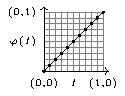
\includegraphics[width=\textwidth]{figures/dyn-prog-full-disc-id/fig.pdf}
        \caption{}
        \label{fig:dyn-prog-full-disc-id}
    \end{subfigure}
    \hfill
    \begin{subfigure}[b]{0.45\textwidth}
        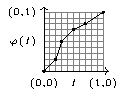
\includegraphics[width=\textwidth]{figures/dyn-prog-full-disc/fig.pdf}
        \caption{}
        \label{fig:dyn-prog-full-disc}
    \end{subfigure}
    \caption[Reparameterization with Full Discretization]{Reparameterization using full discretization. (a) the identity transformation (no change to the original parameterization), and (b) a reparameterized path.}
    \label{fig:dyn-prog}
\end{figure}

The condition \(k < i\) and \(l < j\) ensures the transformation proceeds positively, avoiding loops and maintaining the orientation of \(q_2\).
\subsection{Neighborhood Search Strategy}
\label{subsec:neighborhood-search-strategy}

Despite its straightforward implementation, this method presents significant computational challenges. For a grid comprising \(n \times n\) points, the process involves solving \(n^2\) subproblems, each requiring \(\mathcal{O}(n^2)\) operations. This leads to a total computational complexity of \(\mathcal{O}(n^4)\), making the method computationally intensive, especially for large-scale applications.

To mitigate these computational demands, a strategic limitation of the search area for each subproblem is proposed, as illustrated in Figure \ref{fig:dyn-prog-full-disc-search}. The size of this area must be adaptable based on the grid's dimensions; a fixed size may excessively restrict path movement in smaller grids. Employing this neighborhood search strategy significantly reduces computational cost to \(\mathcal{O}(n^2 |\mathcal{N}(n)|)\), where \(|\mathcal{N}(n)|\) indicates the search area's size.

\begin{figure}
    \centering
    \begin{subfigure}{.3\textwidth}
        \centering
        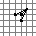
\includegraphics[width=\linewidth]{figures/dyn-prog-full-disc-search-2/fig.pdf}
        \caption{}
        \label{fig:dyn-prog-full-disc-search-2}
    \end{subfigure}%
    \begin{subfigure}{.3\textwidth}
        \centering
        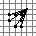
\includegraphics[width=\linewidth]{figures/dyn-prog-full-disc-search-3/fig.pdf}
        \caption{}
        \label{fig:dyn-prog-full-disc-search-3}
    \end{subfigure}%
    \begin{subfigure}{.3\textwidth}
        \centering
        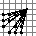
\includegraphics[width=\linewidth]{figures/dyn-prog-full-disc-search-4/fig.pdf}
        \caption{}
        \label{fig:dyn-prog-full-disc-search-4}
    \end{subfigure}
    \caption[Search Areas for Fully Discretized Reparameterization]{Visualization of limited search areas for different values of search depth \(m\): (a) \(m = 2\), (b) \(m = 3\), and (c) \(m = 4\). These figures demonstrate how increasing search depths expand the area being considered, thereby influencing the computational cost and efficiency of the reparameterization process.}    
    \label{fig:dyn-prog-full-disc-search}
\end{figure}

The limited search area is defined as follows:
\begin{equation}
    \mathcal{N}_{(i, j)}(n) = \{(k, l) \mid i-m \leq k < i, \, j-m < l < j, \, \gcd(i - k, j - l) = 1\},
    \label{eq:search-area}
\end{equation}
where \(m = f(n) \in \mathbb{N}^+\) is a function of the grid size \(n\) that determines the extent of the search area. The condition \(\gcd(i - k, j - l) = 1\) ensures that the path does not traverse any intermediate grid points, maintaining a direct route between the specified points and improving the computational efficiency of the process.

To illustrate the implementation of this strategy, we present the pseudocode for the optimal reparameterization process using dynamic programming in Algorithm \ref{alg:optimal-reparam-dp}. This algorithm aligns two curves by optimizing the parameterizations of the second curve, reducing the computational complexity through the limited search area defined earlier.

\begin{algorithm}
    \caption{Optimal Reparameterization via Dynamic Programming}
    \label{alg:optimal-reparam-dp}
    \begin{algorithmic}[1]
    \Require $c_1, c_2$: Curves, $I_1, I_2 \in \mathbb{R}$: Initial parameterizations
    \Function{OptimizeReparam}{$c_1, c_2, I_1, I_2$}
        \State $(I, c_1', c_2') \gets \text{AlignCurves}(c_1, c_2, I_1, I_2)$
        \State $(c_{1,e}', c_{2,e}') \gets \text{MoveStartToIdentity}(c_1', c_2')$ \Comment{\eqref{eq:maurer-cartan-gl}}
        \State $(q_1, q_2) \gets \text{vee}(\text{SRVT}(c_{1,e}', c_{2,e}'))$ \Comment{\eqref{eq:srvt-discrete}, \eqref{eq:vee_SO3}, \eqref{eq:vee_SE3}}
        \State $A, P \gets \text{ComputeCostMatrix}(q_1, q_2)$  \Comment{\eqref{eq:cost-matrix}}
        \State $\text{path} \gets \text{TraceOptimalPath}(P)$ 
        \State $I_{2, opt} \gets \text{LinearInterpolate}(\text{path}_x, \text{path}_y)(I_2)$ 
        \State $c_{2, opt} \gets \text{Interpolate}(I_{2}, I_{2, opt})(c_2)$  \Comment{\eqref{eq:interpolation-discrete}}
        \State \Return $(c_{2, opt}, I_{2, opt})$
    \EndFunction
    \end{algorithmic}
\end{algorithm}

The algorithm detailed in Algorithm \ref{alg:calculate-cost-parent} calculates the cost and parent matrices used in the dynamic programming approach. By leveraging the limited search area, it ensures efficient computation of the optimal path.

\begin{algorithm}
    \caption{Calculate Cost and Parent Matrices for Dynamic Programming}
    \label{alg:calculate-cost-parent}
    \begin{algorithmic}[1]
    \Require $I \in \mathbb{R}^n$: Grid points
    \Require $q_0, q_1 \in \mathbb{R}^{n-1}$: Values defined on the domain of $I$
    \Require $\text{depth} \in \mathbb{N}^+$: Depth of the search area
    \Function{calculateCostMatrixAndParent}{$I, q_0, q_1, \text{depth}$}
        \State $n \gets \text{length}(I)$
        \State $A \gets \text{matrix\_of\_infinity}(n, n)$ \Comment{Initialize cost matrix to a large value}
        \State $P \gets \text{empty matrix}(n, n)$ \Comment{Initialize parent matrix}
        
        \State $A[0, 0] \gets 0$ \Comment{Set initial cost to zero}
        \State $P[0, 0] \gets \text{None}$ \Comment{No predecessor for initial condition}
        
        \For{$i \gets 0$ \textbf{to} $n-1$}
            \For{$j \gets 0$ \textbf{to} $n-1$}
                \State $\text{preds} \gets \text{findPreds}(i, j, \text{depth})$ \Comment{\eqref{eq:search-area}}
                \For{$\text{pred} \in \text{preds}$}
                    \State $\text{cost\_to\_pred} \gets \text{localCost}(i, j, \text{pred}, q_0, q_1)$ 
                    \Comment{\eqref{eq:local-cost-functional}, \eqref{eq:local-cost-functional-SE3}}
                    \State $\text{cost} \gets \text{cost\_to\_pred} + A[\text{pred}]$ \Comment{\eqref{eq:cost-matrix}}
                    \If{$\text{cost} < A[i, j]}$
                        \State $A[i, j] \gets \text{cost}$
                        \State $P[i, j] \gets \text{pred}$
                    \EndIf
                \EndFor
            \EndFor
        \EndFor
    
        \State \Return $P, A$
    \EndFunction
    \end{algorithmic}
\end{algorithm}
\subsection{Synthetic Data Generation}
\label{subsec:synthetic-data-generation}

In this subsection, we outline the process of generating synthetic data for numerical analysis. This synthetic data is critical for evaluating our reparameterization framework. We generate data by solving differential equations with different parameterizations. The synthetic data includes trajectories, parameterizations, and curves for different groups such as \(\mathrm{SO}(3)\), \(\mathrm{SE}(3)\), \(\mathrm{SO}(3)^3\), and \(\mathrm{SE}(3)^3\). These elements are used later in our numerical analysis.

\subsubsection{Generating Synthetic Trajectories}
\label{subsubsec:synthetic-trajectories-generation}

To generate synthetic trajectories, we model the system using the differential equation:
\begin{equation}
    \frac{d}{dt} g(t) = g(t) \hat{u}(t), \quad t \in [0, 1],
    \label{eq:diff-eq-synthetic}
\end{equation}
where \( g(t) \in \mathrm{SO}(3) \) or \( \mathrm{SE}(3) \), and \(\hat{u}(t)\) is the hat map of \(u(t)\). We assume an initial value \( g(0) = e \) (the identity element). By varying \(\hat{u}(t)\) with different parameterizations, we synthesize diverse datasets. The trajectories are approximated using the fourth-order Runge-Kutta (RK4) method \cite{rungeUeberNumerischeAufloesung1895,butcherCoefficientsStudyRungeKutta1963} over discrete time intervals.

For \(\mathrm{SO}(3)\), we set \(u(t) = \omega_i(t) \in \mathbb{R}^3\). For \(\mathrm{SE}(3)\), we set \(u(t) = \xi_i(t) = [\omega_i(t), v_i(t)]^T \in \mathbb{R}^6\), which is mapped to the corresponding Lie algebra via \eqref{eq:hat_SO3} and \eqref{eq:hat_SE3}.

To demonstrate the generation of synthetic data for Cartesian curves, \(n = 3\) is chosen. For either \(\mathrm{SO}(3)^3\) or \(\mathrm{SE}(3)^3\), we define three different functions \(u(t)\). Thus, solving \eqref{eq:diff-eq-synthetic} generates three synthetic trajectories over discrete time intervals.

We define nine \(\omega_i(t)\) and nine \(v_i(t)\) to generate the rotational and translational components, respectively, used for \(u(t)\). The rotational functions are defined in \eqref{eq:synthetic-data-rotation}, and the translational functions are defined in \eqref{eq:synthetic-data-translation}.

\begin{equation}
    \begin{aligned}
        \omega_1(t) &= 
            [2 \sin(3t) \exp(t), 4 \cos(3t), 3t \sin(t) \cos(t)]^T \\
        \omega_2(t) &= 
            [3t, 4 \sin(10t), 3t \sin(t) \cos(t)]^T \\
        \omega_3(t) &= 
            [4t^2, 5 \sin(4t) \sin(6t), 3t \cos(t)]^T \\
        \omega_4(t) &= 
            [3 \sin(2t) \exp(-t), 5 \cos(2t), 4t \sin(t) \cos(t)]^T \\
        \omega_5(t) &= 
            [t^3, 5 \sin(5t), 2t \sin(t) \sin(t)]^T \\
        \omega_6(t) &= 
            [2t^2, 3 \sin(6t) \cos(t), 5t \cos(t) \cos(t)]^T \\
        \omega_7(t) &= 
            [-1, 6 \sin(3t), 3t \sin(t)]^T \\
        \omega_8(t) &= 
            [t^2, 4 \cos(3t), t \sin(t)]^T \\
        \omega_9(t) &= 
            [3t, 5 \sin(2t), 2t \cos(t)]^T
    \end{aligned}
    \label{eq:synthetic-data-rotation}
\end{equation}

\begin{equation}
    \begin{aligned}
        v_1(t) &= 
        [3t \sin(t) \cos(t), t, \cos(t), \sin(3t)]^T \\
        v_2(t) &=
        [\sin(2t), \cos(3t), \exp(t)]^T \\
        v_3(t) &=
        [\cos(t) \cos(3t), \sin(4t), \cos(2t)]^T \\
        v_4(t) &=
        [t^2, \sin(t^2), \exp(-t)]^T \\
        v_5(t) &=
        [\cos(2t), \log(t + 1), t]^T \\
        v_6(t) &=
        [\sin(t) \cos(t), t^3, \sin(t^3)]^T \\
        v_7(t) &=
        [\cos(5t), \exp(t/2), t \sin(t)]^T \\
        v_8(t) &=
        [\sin(2t), t \exp(-t), \cos(t^2)]^T \\
        v_9(t) &=
        [t^2 \cos(t), \sin(t^2), -0.5]^T
    \end{aligned}
    \label{eq:synthetic-data-translation}
\end{equation}

By solving \eqref{eq:diff-eq-synthetic} with \(u(t) = \omega_i(t)\), for \(i = 1, 2, \dots, 9\) over equidistant points on \([0,1]\), we obtain the rotational trajectories depicted in Figure \ref{fig:synthetic-rotation}. Similarly, by solving \eqref{eq:diff-eq-synthetic} with \(u(t) = \xi_i(t)\), for \(i = 1, 2, \dots, 9\) over equidistant points on \([0,1]\), and extracting the positions, we generate the translation plot shown in Figure \ref{fig:synthetic-translation}. These plots provide a clear visual representation of the varied rotational and translational paths used later in the analysis. The rotations are plotted on spheres, representing pure rotational movements.

\newpage
\begin{figure}
    \centering
    \foreach \i in {1,...,9} {
        \begin{subfigure}{0.26\textwidth}
            \includegraphics[width=\textwidth]{figures/syntetic_data/SO3_fig\i.png}
            \caption{}
            \label{fig:synthetic-SO3-fig\i}
        \end{subfigure}
        \ifnum\i=3
            \par\medskip % start a new line after the third subfigure
        \fi
        \ifnum\i=6
            \par\medskip % start a new line after the sixth subfigure
        \fi
    }
    \caption[Visualization of Rotations from Synthetic Data]{Rotations generated from synthetic data using \eqref{eq:synthetic-data-rotation}. Each subfigure (a-i) shows the rotation of the initial vector \([0, 0, 1]\) governed by \eqref{eq:diff-eq-synthetic} with \(\hat{u}(t) = \hat{\omega}_i(t)\), evaluated over \([0, 1]\) with 100 time points. Subfigures (a-i) correspond to \(i = 1\) to \(i = 9\), respectively.}
    \label{fig:synthetic-rotation}
\end{figure}

\newpage
\begin{figure}
    \centering
    \foreach \i in {1,2,3,4,5,6,7,8,9} {
        \begin{subfigure}[b]{0.3\textwidth}
            \centering
            \begin{tikzpicture}
                \begin{axis}[
                    height=4.5cm,
                    width=5cm,
                    xlabel=$x$, 
                    ylabel=$y$, 
                    zlabel=$z$,
                    ytick=\empty,
                    xtick=\empty,
                    ztick=\empty
                ]
                    \addplot3+[
                        mark options={red, mark size=0.5pt},
                        only marks,
                    ] table [col sep=comma, x=x, y=y, z=z] {figures/syntetic_data/SE3_t_\i.csv};
                \end{axis}
            \end{tikzpicture}
            \caption{}
        \end{subfigure}
        \ifnum\i=3 \hspace{0pt}\par\fi % Line break after every third subfigure
        \ifnum\i=6 \hspace{0pt}\par\fi
    }
    \caption[Visualization of Translations from Synthetic Data]{Translation part of the \(\mathrm{SE}(3)\) elements generated from synthetic data by solving \eqref{eq:diff-eq-synthetic} with the functions defined in \eqref{eq:synthetic-data-rotation} and \eqref{eq:synthetic-data-translation}. Each subfigure (a-i) illustrates the translation governed by \eqref{eq:diff-eq-synthetic} with \(\hat{u}(t) = \hat{\xi}_i(t)\), evaluated over \([0, 1]\) with 100 time points. Subfigures (a-i) correspond to \(i = 1\) to \(i = 9\), respectively.}
    \label{fig:synthetic-translation}
\end{figure}

\FloatBarrier
\subsubsection{Generate Synthetic Parameterizations}
\label{subsubsec:generate-synthetic-parameterizations}

We generate three distinct synthetic parameterizations, each created by \(\varphi(x) \in \mathrm{Diff}^+([0,1])\):

\begin{equation}
    \varphi(x) = x + F(x),
\end{equation}
where \(\varphi'(x) = 1 + F'(x) > 0\). The function \(F(x)\) is constructed using an orthogonal sine basis function \(\psi_n(x)\):

\begin{equation}
    \psi_n(x) = \frac{\sin(n \pi x)}{n \pi}, \quad n \in \mathbb{N}.
\end{equation}

These basis functions are orthogonal over \([0, 1]\) and vanish at the endpoints, making them suitable for weighted sums. Consequently, \(F(x)\) is represented as:

\begin{equation}
    F(x) = \sum_{n=1}^{M} w_n \psi_n(x) = \sum_{n=1}^{M} w_n \frac{\sin(n \pi x)}{n \pi},
\end{equation}
where \(w_n\) are the weights associated with each basis function. The derivative \(F'(x)\) is:

\begin{equation}
    F'(x) = \sum_{n=1}^{M} w_n \cos(n \pi x).
\end{equation}

Since each cosine term is bounded by 1, the derivative \(F'(x)\) satisfies:

\begin{equation}
    |F'(x)| \leq \|\mathbf{w}\|_1.
\end{equation}

Therefore, the derivative of \(\varphi(x)\) is:

\begin{equation}
    \varphi'(x) = 1 + \sum_{n=1}^{M} w_n \cos(n \pi x).
\end{equation}

To ensure \(\varphi'(x) > 0\), we scale \(F(x)\) by a factor \(\frac{1 - \epsilon}{\|\mathbf{w}\|_1}\), where \(\epsilon\) is a small positive number. This guarantees that the sum of the cosine terms is less than 1, ensuring \(\varphi'(x) > 0\):

\begin{equation}
    1 + \sum_{n=1}^{M} w_n \frac{1 - \epsilon}{\|\mathbf{w}\|_1} \cos(n \pi x) > 0.
\end{equation}

The synthetic parameterizations generated using this method are illustrated in Figure \ref{fig:synthetic-parameterizations}. For this, we set \(M = 4\), initialize the weights \(w_n\) with a normal distribution \(\mathcal{N}(0, 2)\), and use 100 equidistant steps with a tolerance of \(\epsilon = 10^{-8}\).

\begin{figure}
    \begin{tikzpicture}
        \begin{axis}[
            width=0.7\textwidth,
            height=0.5\textwidth,
            xlabel={\( x \)},
            ylabel={\( \varphi(x) \)},
            grid=major,
            grid style={dashed,gray!30},
            legend style={at={(1.05,0.5)}, anchor=west},
            line width=1pt,
            xmin=0, xmax=1,
            ymin=0, ymax=1
        ]
        \addplot [smooth, thick, red] table [x=x, y=varphi_1, col sep=comma] {figures/syntetic_data/parameterization/varphi_1.csv};
        \addlegendentry{\( \varphi_1 \)}
        \addplot [smooth, thick, blue] table [x=x, y=varphi_2, col sep=comma] {figures/syntetic_data/parameterization/varphi_2.csv};
        \addlegendentry{\( \varphi_2 \)}
        \addplot [smooth, thick, orange] table [x=x, y=varphi_3, col sep=comma] {figures/syntetic_data/parameterization/varphi_3.csv};
        \addlegendentry{\( \varphi_3 \)}
        \end{axis}
    \end{tikzpicture}    
    \caption[Visualization of the Synthetic Parameterizations]{Visualization of three distinct synthetic parameterizations generated by setting \(M = 4\), initializing the weights \(w_n\) with a normal distribution \(\mathcal{N}(0, 2)\), and using 100 equidistant steps with a tolerance of \(\epsilon = 10^{-8}\).}
    \label{fig:synthetic-parameterizations}
\end{figure}

\FloatBarrier
\subsubsection{Generate Synthetic Curves}
\label{subsubsec:synthetic-curves}

To evaluate our reparameterization framework, we generate synthetic curves by solving Equation \eqref{eq:diff-eq-synthetic} with the parameterizations \(\varphi_1, \varphi_2, \varphi_3\) described in Section \ref{subsubsec:generate-synthetic-parameterizations}, as well as an equidistant parameterization. This differential equation is solved using the functions defined in Equations \eqref{eq:synthetic-data-rotation} and \eqref{eq:synthetic-data-translation}, which provide \(u(t) = \omega_i(t)\) for \(\mathrm{SO}(3)\) elements and \(u(t) = \xi_i(t) = [\omega_i(t), v_i(t)]^T\) for \(\mathrm{SE}(3)\) elements, where \(i = 1,2,3\). This process creates single-element and three-element Cartesian curves, with each group comprising three shapes, each represented under four different parameterizations, yielding twelve curves per group.

For multi-component groups \(\mathrm{SO}(3)^3\) and \(\mathrm{SE}(3)^3\), we define composite parameters:
\begin{gather}
    \omega_{i, i+1, i+2} = [\omega_i, \omega_{i+1}, \omega_{i+2}], \nonumber \\
    \xi_{i, i+1, i+2} = \left[ \xi_i, \xi_{i+1}, \xi_{i+2} \right] = \left[ [\omega_i, v_i], [\omega_{i+1}, v_{i+1}], [\omega_{i+2}, v_{i+2}] \right] 
\end{gather}
for \(i \in \{1, 4, 7\}\).

The idea is to create three interconnected curves that together form a single composite curve. These parameters are used to solve the differential equation under the same parameterizations, generating twelve curves per group. Each group of four curves shares identical geometric shapes, differentiated by parameterization.

The notation for the curves is as follows: single-element curves are denoted \(c_i^j\), where \(i\) indicates the parameter used (\(\omega_i\) or \(\xi_i = [\omega_i, v_i]\)) and \(j\) the specific parameterization (\(\varphi_j\)). Curves generated using the equidistant parameterization are denoted as \(c_i^{\text{eq}}\). Cartesian curves are expressed as \(c_{i, i+1, i+2}^j\) for individual parameterizations and \(c_{i, i+1, i+2}^{\text{eq}}\) for the equidistant parameterization.

\subsection{Numerical Analysis}
\label{sec:numerical-reparameterization}

In this subsection we will use the data in \ref{subsec:synthetic-data-generation} perform reparameterization, classification and measure performance in terms of accuracy and computation time as the search size increases.

\FloatBarrier
\subsubsection{Reparameterization of Curves}
\label{subsec:reparameterization-curves}

In this subsection, we evaluate the reparameterization framework using synthetic curves generated previously (Section \ref{subsec:synthetic-data-generation}). The goal is to reparameterize the equidistantly parameterized curves \(c_i^\text{eq}\) into the curves \(c_i^j\) for \(i \in \{1, 2, 3\}\) and \(c_{i,i+1,i+2}^\text{eq}\) into the curves \(c_{i,i+1,i+2}^j\) for \(i \in \{1, 4, 7\}\), for all parameterizations \(j \in \{1, 2, 3\}\). This evaluation checks whether we can find the optimal reparameterization when the shapes are the same, demonstrating that we can effectively remove the effects of parameterization through reparameterization. It does not, however, determine whether we can differentiate between different shapes.

The objective is to find the optimal reparameterization \(\hat{\varphi}_j\) that approximates \(\varphi_j\). The relationship between the curves is given by:
\begin{equation}
    c_i^j = c_i^\text{eq} \circ \varphi_j
\end{equation}

Hence, each curve \(c_i^j\) is obtained by composing the equidistant curve \(c_i^\text{eq}\) with one of the parameterizations \(\varphi_1, \varphi_2\), or \(\varphi_3\). Thus, to find the optimal reparameterization \(\hat{\varphi}_j\), we minimize the distance \(d_{\mathcal{S}_*}\) between \(c_i^j\) and \(c_i^{\text{eq}}\):
\begin{equation}
    d_{\mathcal{S}_*}(c_i^j, c_i^{\text{eq}}) = \min_{\hat{\varphi}_j} d_{\mathcal{P}_*}(c_i^{\text{eq}} \circ \varphi_j, c_i^{\text{eq}} \circ \hat{\varphi}_j)
\end{equation}

This minimization process helps to determine \(\hat{\varphi}_j\) such that \(\hat{\varphi}_j \approx \varphi_j\), indicating that the reparameterization framework can effectively approximate the original parameterizations.

The results after reparameterization for the curves in \(\mathrm{SO}(3)\), \(\mathrm{SE}(3)\), \(\mathrm{SO}(3)^3\), and \(\mathrm{SE}(3)^3\) are presented in Figures \ref{fig:reparameterization-SO3}, \ref{fig:reparameterization-SE3}, \ref{fig:reparameterization-SO3-3}, and \ref{fig:reparameterization-SE3-3}, respectively.

\begin{figure}
    \begin{tikzpicture}
        \begin{axis}[
            width=0.85\textwidth,
            height=0.55\textwidth,
            xlabel={\( x \)},
            ylabel={\( \varphi(x) \)},
            grid=major,
            grid style={dashed,gray!30},
            legend style={at={(1.05,0.5)}, anchor=west},
            line width=1pt,
            xmin=0, xmax=1,
            ymin=0, ymax=1,
        ]
        \addplot [thin, red, solid] table [x=x, y=varphi_1, col sep=comma] {figures/syntetic_data/parameterization/varphi_1.csv};
        \addlegendentry{\( \varphi_1\)}

        \addplot [thin, blue, solid] table [x=x, y=varphi_2, col sep=comma] {figures/syntetic_data/parameterization/varphi_2.csv};
        \addlegendentry{\( \varphi_2\)}

        \addplot [thin, green, solid] table [x=x, y=varphi_3, col sep=comma] {figures/syntetic_data/parameterization/varphi_3.csv};
        \addlegendentry{\( \varphi_3\)}


        \addplot [red, dashed] table [x=x, y=g0, col sep=comma] {figures/syntetic_data/reparameterization_SO3/df_varphi_1.csv};
        \addlegendentry{\( \hat \varphi_{1}^{1}\)}

        \addplot [red, dotted] table [x=x, y=g1, col sep=comma] {figures/syntetic_data/reparameterization_SO3/df_varphi_1.csv};
        \addlegendentry{\( \hat \varphi_{1}^{2}\)}

        \addplot [red, dashdotted] table [x=x, y=g2, col sep=comma] {figures/syntetic_data/reparameterization_SO3/df_varphi_1.csv};
        \addlegendentry{\( \hat \varphi_{1}^{3}\)}

        \addplot [blue, dashed] table [x=x, y=g0, col sep=comma] {figures/syntetic_data/reparameterization_SO3/df_varphi_2.csv};
        \addlegendentry{\( \hat \varphi_{2}^{1}\)}

        \addplot [blue, dotted] table [x=x, y=g1, col sep=comma] {figures/syntetic_data/reparameterization_SO3/df_varphi_2.csv};
        \addlegendentry{\( \hat \varphi_{2}^{2}\)}

        \addplot [blue, dashdotted] table [x=x, y=g2, col sep=comma] {figures/syntetic_data/reparameterization_SO3/df_varphi_2.csv};
        \addlegendentry{\( \hat \varphi_{2}^{3}\)}

        \addplot [green, dashed] table [x=x, y=g0, col sep=comma] {figures/syntetic_data/reparameterization_SO3/df_varphi_3.csv};
        \addlegendentry{\( \hat \varphi_{3}^{1}\)}

        \addplot [green, dotted] table [x=x, y=g1, col sep=comma] {figures/syntetic_data/reparameterization_SO3/df_varphi_3.csv};
        \addlegendentry{\( \hat \varphi_{3}^{2}\)}

        \addplot [green, dashdotted] table [x=x, y=g2, col sep=comma] {figures/syntetic_data/reparameterization_SO3/df_varphi_3.csv};
        \addlegendentry{\( \hat \varphi_{3}^{3}\)}

        \end{axis}
    \end{tikzpicture}    
    \caption[Reparameterization of curves in \(\mathrm{SO}(3)\)]{Comparison of reparameterized curves \(\hat{\varphi}_j^i\) with the analytical parameterizations \(\varphi_j\) for curves in \(\mathrm{SO}(3)\). The curves \(c_i^{\text{eq}}\) have been fitted to \(c_i^j\) for \(j = 1, 2, 3\), and for all shapes \(i = 1, 2, 3\). Optimal reparameterizations are indicated by \(\hat{\varphi}_i^j\) being close to \(\varphi_j\).}
    \label{fig:reparameterization-SO3}
\end{figure}

\begin{figure}
    \begin{tikzpicture}
        \begin{axis}[
            width=0.85\textwidth,
            height=0.55\textwidth,
            xlabel={\( x \)},
            ylabel={\( \varphi(x) \)},
            grid=major,
            grid style={dashed,gray!30},
            legend style={at={(1.05,0.5)}, anchor=west},
            line width=1pt,
            xmin=0, xmax=1,
            ymin=0, ymax=1,
        ]
        \addplot [thin, red, solid] table [x=x, y=varphi_1, col sep=comma] {figures/syntetic_data/parameterization/varphi_1.csv};
        \addlegendentry{\( \varphi_1\)}

        \addplot [thin, blue, solid] table [x=x, y=varphi_2, col sep=comma] {figures/syntetic_data/parameterization/varphi_2.csv};
        \addlegendentry{\( \varphi_2\)}

        \addplot [thin, green, solid] table [x=x, y=varphi_3, col sep=comma] {figures/syntetic_data/parameterization/varphi_3.csv};
        \addlegendentry{\( \varphi_3\)}

        \addplot [red, dashed] table [x=x, y=g0, col sep=comma] {figures/syntetic_data/reparameterization_SE3/df_varphi_1.csv};
        \addlegendentry{\( \hat \varphi_{1}^1\)}

        \addplot [red, dotted] table [x=x, y=g1, col sep=comma] {figures/syntetic_data/reparameterization_SE3/df_varphi_1.csv};
        \addlegendentry{\( \hat \varphi_{1}^2\)}

        \addplot [red, dashdotted] table [x=x, y=g2, col sep=comma] {figures/syntetic_data/reparameterization_SE3/df_varphi_1.csv};
        \addlegendentry{\( \hat \varphi_{1}^3\)}

        \addplot [blue, dashed] table [x=x, y=g0, col sep=comma] {figures/syntetic_data/reparameterization_SE3/df_varphi_2.csv};
        \addlegendentry{\( \hat \varphi_{2}^1\)}

        \addplot [blue, dotted] table [x=x, y=g1, col sep=comma] {figures/syntetic_data/reparameterization_SE3/df_varphi_2.csv};
        \addlegendentry{\( \hat \varphi_{2}^2\)}

        \addplot [blue, dashdotted] table [x=x, y=g2, col sep=comma] {figures/syntetic_data/reparameterization_SE3/df_varphi_2.csv};
        \addlegendentry{\( \hat \varphi_{2}^3\)}

        \addplot [green, dashed] table [x=x, y=g0, col sep=comma] {figures/syntetic_data/reparameterization_SE3/df_varphi_3.csv};
        \addlegendentry{\( \hat \varphi_{3}^1\)}

        \addplot [green, dotted] table [x=x, y=g1, col sep=comma] {figures/syntetic_data/reparameterization_SE3/df_varphi_3.csv};
        \addlegendentry{\( \hat \varphi_{3}^2\)}

        \addplot [green, dashdotted] table [x=x, y=g2, col sep=comma] {figures/syntetic_data/reparameterization_SE3/df_varphi_3.csv};
        \addlegendentry{\( \hat \varphi_{3}^3\)}

        \end{axis}
    \end{tikzpicture}    
    \caption[Reparameterization of curves in \(\mathrm{SE}(3)\)]{Comparison of reparameterized curves \(\hat{\varphi}_j^i\) with the analytical parameterizations \(\varphi_j\) for curves in \(\mathrm{SE}(3)\). The curves \(c_i^{\text{eq}}\) have been fitted to \(c_i^j\) for \(j = 1, 2, 3\), and for all shapes \(i = 1, 2, 3\). Optimal reparameterizations are indicated by \(\hat{\varphi}_j^i\) being close to \(\varphi_j\).}
    \label{fig:reparameterization-SE3}
\end{figure}

\begin{figure}
    \begin{tikzpicture}
        \begin{axis}[
            width=0.8\textwidth,
            height=0.55\textwidth,
            xlabel={\( x \)},
            ylabel={\( \varphi(x) \)},
            grid=major,
            grid style={dashed,gray!30},
            legend style={at={(1.05,0.5)}, anchor=west},
            line width=1pt,
            xmin=0, xmax=1,
            ymin=0, ymax=1,
        ]
        \addplot [thin, red, solid] table [x=x, y=varphi_1, col sep=comma] {figures/syntetic_data/parameterization/varphi_1.csv};
        \addlegendentry{\( \varphi_1\)}

        \addplot [thin, blue, solid] table [x=x, y=varphi_2, col sep=comma] {figures/syntetic_data/parameterization/varphi_2.csv};
        \addlegendentry{\( \varphi_2\)}

        \addplot [thin, green, solid] table [x=x, y=varphi_3, col sep=comma] {figures/syntetic_data/parameterization/varphi_3.csv};
        \addlegendentry{\( \varphi_3\)}


        \addplot [red, dashed] table [x=x, y=g0, col sep=comma] {figures/syntetic_data/reparameterization_SO3_3/df_varphi_1.csv};
        \addlegendentry{\( \hat \varphi_{1}^{(1,2,3)}\)}

        \addplot [red, dotted] table [x=x, y=g1, col sep=comma] {figures/syntetic_data/reparameterization_SO3_3/df_varphi_1.csv};
        \addlegendentry{\( \hat \varphi_{1}^{(4,5,6)}\)}

        \addplot [red, dashdotted] table [x=x, y=g2, col sep=comma] {figures/syntetic_data/reparameterization_SO3_3/df_varphi_1.csv};
        \addlegendentry{\( \hat \varphi_{1}^{(7,8,9)}\)}

        \addplot [blue, dashed] table [x=x, y=g0, col sep=comma] {figures/syntetic_data/reparameterization_SO3_3/df_varphi_2.csv};
        \addlegendentry{\( \hat \varphi_{2}^{(1,2,3)}\)}

        \addplot [blue, dotted] table [x=x, y=g1, col sep=comma] {figures/syntetic_data/reparameterization_SO3_3/df_varphi_2.csv};
        \addlegendentry{\( \hat \varphi_{2}^{(4,5,6)}\)}

        \addplot [blue, dashdotted] table [x=x, y=g2, col sep=comma] {figures/syntetic_data/reparameterization_SO3_3/df_varphi_2.csv};
        \addlegendentry{\( \hat \varphi_{2}^{(7,8,9)}\)}

        \addplot [green, dashed] table [x=x, y=g0, col sep=comma] {figures/syntetic_data/reparameterization_SO3_3/df_varphi_3.csv};
        \addlegendentry{\( \hat \varphi_{3}^{(1,2,3)}\)}

        \addplot [green, dotted] table [x=x, y=g1, col sep=comma] {figures/syntetic_data/reparameterization_SO3_3/df_varphi_3.csv};
        \addlegendentry{\( \hat \varphi_{3}^{(4,5,6)}\)}

        \addplot [green, dashdotted] table [x=x, y=g2, col sep=comma] {figures/syntetic_data/reparameterization_SO3_3/df_varphi_3.csv};
        \addlegendentry{\( \hat \varphi_{3}^{(7,8,9)}\)}
        \end{axis}
    \end{tikzpicture}    
    \caption[Reparameterization of curves in \(\mathrm{SO}(3)^3\)]{Comparison of reparameterized curves \(\hat{\varphi}_j^{i,i+1,i+2}\) with the analytical parameterizations \(\varphi_j\) for curves in \(\mathrm{SE}(3)\). The curves \(c_{i,i+1,i+2}^{\text{eq}}\) have been fitted to \(c_{i,i+1,i+2}^j\) for \(i \in \{1, 2, 3\}\), and for all shapes \(i \in \{1, 4, 7\}\). Optimal reparameterizations are indicated by \(\hat{\varphi}_j^{i,i+1,i+2}\) being close to \(\varphi_j\).}
    \label{fig:reparameterization-SO3-3}
\end{figure}

\begin{figure}
    \begin{tikzpicture}
        \begin{axis}[
            width=0.8\textwidth,
            height=0.55\textwidth,
            xlabel={\( x \)},
            ylabel={\( \varphi(x) \)},
            grid=major,
            grid style={dashed,gray!30},
            legend style={at={(1.05,0.5)}, anchor=west},
            line width=1pt,
            xmin=0, xmax=1,
            ymin=0, ymax=1,
        ]
        \addplot [thin, red, solid] table [x=x, y=varphi_1, col sep=comma] {figures/syntetic_data/parameterization/varphi_1.csv};
        \addlegendentry{\( \varphi_1\)}

        \addplot [thin, blue, solid] table [x=x, y=varphi_2, col sep=comma] {figures/syntetic_data/parameterization/varphi_2.csv};
        \addlegendentry{\( \varphi_2\)}

        \addplot [thin, green, solid] table [x=x, y=varphi_3, col sep=comma] {figures/syntetic_data/parameterization/varphi_3.csv};
        \addlegendentry{\( \varphi_3\)}



        \addplot [red, dashed] table [x=x, y=g0, col sep=comma] {figures/syntetic_data/reparameterization_SE3_3/df_varphi_1.csv};
        \addlegendentry{\( \hat \varphi_{1}^{(1,2,3)}\)}

        \addplot [red, dotted] table [x=x, y=g1, col sep=comma] {figures/syntetic_data/reparameterization_SE3_3/df_varphi_1.csv};
        \addlegendentry{\( \hat \varphi_{1}^{(4,5,6)}\)}

        \addplot [red, dashdotted] table [x=x, y=g2, col sep=comma] {figures/syntetic_data/reparameterization_SE3_3/df_varphi_1.csv};
        \addlegendentry{\( \hat \varphi_{1}^{(7,8,9)}\)}

        \addplot [blue, dashed] table [x=x, y=g0, col sep=comma] {figures/syntetic_data/reparameterization_SE3_3/df_varphi_2.csv};
        \addlegendentry{\( \hat \varphi_{2}^{(1,2,3)}\)}

        \addplot [blue, dotted] table [x=x, y=g1, col sep=comma] {figures/syntetic_data/reparameterization_SE3_3/df_varphi_2.csv};
        \addlegendentry{\( \hat \varphi_{2}^{(4,5,6)}\)}

        \addplot [blue, dashdotted] table [x=x, y=g2, col sep=comma] {figures/syntetic_data/reparameterization_SE3_3/df_varphi_2.csv};
        \addlegendentry{\( \hat \varphi_{2}^{(7,8,9)}\)}

        \addplot [green, dashed] table [x=x, y=g0, col sep=comma] {figures/syntetic_data/reparameterization_SE3_3/df_varphi_3.csv};
        \addlegendentry{\( \hat \varphi_{3}^{(1,2,3)}\)}

        \addplot [green, dotted] table [x=x, y=g1, col sep=comma] {figures/syntetic_data/reparameterization_SE3_3/df_varphi_3.csv};
        \addlegendentry{\( \hat \varphi_{3}^{(4,5,6)}\)}

        \addplot [green, dashdotted] table [x=x, y=g2, col sep=comma] {figures/syntetic_data/reparameterization_SE3_3/df_varphi_3.csv};
        \addlegendentry{\( \hat \varphi_{3}^{(7,8,9)}\)}

        \end{axis}
    \end{tikzpicture}    
    \caption[Reparameterization of curves in \(\mathrm{SE}(3)^3\)]{Comparison of reparameterized curves \(\hat{\varphi}_j^{i,i+1,i+2}\) with the analytical parameterizations \(\varphi_j\) for curves in \(\mathrm{SE}(3)\). The curves \(c_{i,i+1,i+2}^{\text{eq}}\) have been fitted to \(c_{i,i+1,i+2}^j\) for \(j \in \{1, 2, 3\}\), and for all shapes \(i \in \{1, 4, 7\}\). Optimal reparameterizations are indicated by \(\hat{\varphi}_j^{i,i+1,i+2}\) being close to \(\varphi_j\).}
    \label{fig:reparameterization-SE3-3}
\end{figure}

The reparameterization results show that the optimal reparameterizations \(\hat{\varphi}_j^i\) for \(i \in \{1, 2, 3\}\) and \(\hat{\varphi}_j^{i,i+1,i+2}\) for \(i \in \{1, 4, 7\}\) closely approximate the original parameterizations \(\varphi_j\) for all \(j \in \{1, 2, 3\}\). This indicates that our framework can effectively remove the effects of parameterization. The results are consistent across all groups, attesting to its robustness. However, this evaluation only verifies the ability to find the parameterization for curves with the same shape. 

Overall, the results affirm the reparameterization framework's effectiveness in approximating original parameterizations and suggest its potential for broader applications in shape analysis and related fields.

\FloatBarrier
\subsubsection{Classification of Curves}
\label{subsec:classification-curves}

The primary objective here is to classify curves based on their geometric shapes using our reparameterization framework. This classification utilizes the curves generated in Section \ref{subsec:synthetic-data-generation}. Specifically, we use the curves \(c_i^j\) and \(c_i^{\text{eq}}\) for \(\mathrm{SO}(3)\) and \(\mathrm{SE}(3)\), as well as \(c_{i,i+1,i+2}^j\) and \(c_{i,i+1,i+2}^{\text{eq}}\) for \(\mathrm{SO}(3)^3\) and \(\mathrm{SE}(3)^3\). Our framework aims to find the shape space metric \(d_{\mathcal{S}_*}\), as defined in Equation \eqref{eq:shape-space-metric-id}, between these curves to create a distance matrix. Instead of directly classifying the curves, we visualize the distances to observe clustering of similar shapes and separation of different shapes.

The color map of this matrix highlights the effectiveness of shape-based classification. We expect a block diagonal pattern in the matrix, with three 4x4 blocks along the diagonal indicating lower distances and thus, shape similarities. Conversely, the off-diagonal blocks should display higher, relatively uniform distances, suggesting distinct shapes. This pattern would confirm successful classification based on shape reparameterization, showing that geometrically similar curves cluster together, while different shapes are well-separated. 

\begin{figure}
    \centering
    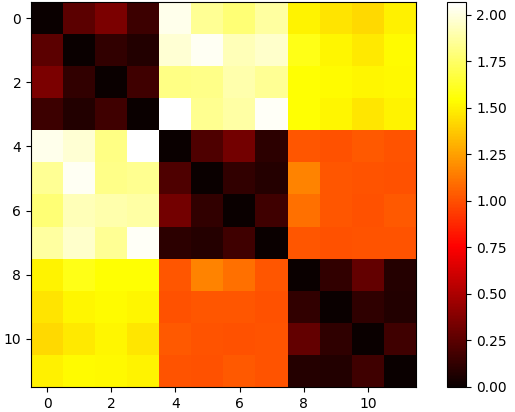
\includegraphics[width=0.7\linewidth]{figures/syntetic_data/distance_matrix/SO3.png}
    \caption[Classification using reparameterization of curves in \(\mathrm{SO}(3)\)]{Heat map of the distance matrix for twelve synthetic \(\mathrm{SO}(3)\) curves, denoted \(c_i^j\), where \(i \in \{1, 2, 3\}\) indicates the shape and \(j \in \{1, 2, 3, \text{eq}\}\) represents the parameterization. The color intensity reflects the shape space distance, with lower distances indicating similarity in shape and higher distances signifying distinct shapes.}
    \label{fig:classification-SO3}
\end{figure}

\begin{figure}
    \centering
    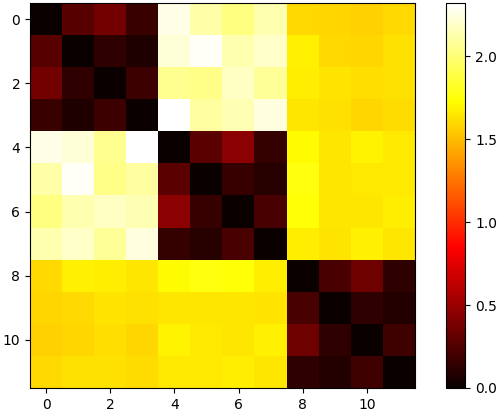
\includegraphics[width=0.7\linewidth]{figures/syntetic_data/distance_matrix/SE3.png}
    \caption[Classification using reparameterization of curves in \(\mathrm{SE}(3)\)]{Heat map of the distance matrix for twelve synthetic \(\mathrm{SE}(3)\) curves, denoted \(c_i^j\), where \(i \in \{1, 2, 3\}\) indicates the shape and \(j \in \{1, 2, 3, \text{eq}\}\) represents the parameterization. The color intensity reflects the shape space distance, with lower distances indicating similarity in shape and higher distances signifying distinct shapes.}
    \label{fig:classification-SE3}
\end{figure}

\begin{figure}
    \centering
    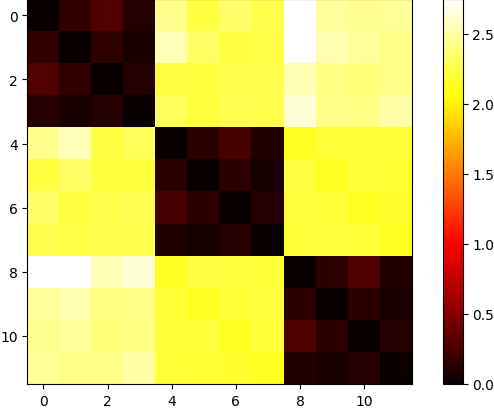
\includegraphics[width=0.7\linewidth]{figures/syntetic_data/distance_matrix/SO3_3.png}
    \caption[Classification using reparameterization of curves in \(\mathrm{SO}(3)^3\)]{Heat map of the distance matrix for twelve synthetic \(\mathrm{SO}(3)^3\) curves, denoted \(c_{(i,i+1,i+2)}^j\), where \(i \in \{1, 4, 7\}\) indicates the shape and \(j \in \{1, 2, 3, \text{eq}\}\) represents the parameterization. The color intensity reflects the shape space distance, with lower distances indicating similarity in shape and higher distances signifying distinct shapes.}
    \label{fig:classification-SO3-3}
\end{figure}

\begin{figure}
    \centering
    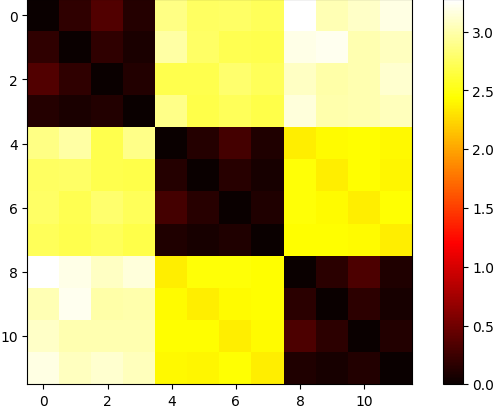
\includegraphics[width=0.7\linewidth]{figures/syntetic_data/distance_matrix/SE3_3.png}
    \caption[Classification using reparameterization of curves in \(\mathrm{SE}(3)^3\)]{Heat map of the distance matrix for twelve synthetic \(\mathrm{SE}(3)^3\) curves, denoted \(c_{(i,i+1,i+2)}^j\), where \(i \in \{1, 4, 7\}\) indicates the shape and \(j \in \{1, 2, 3, \text{eq}\}\) represents the parameterization. The color intensity reflects the shape space distance, with lower distances indicating similarity in shape and higher distances signifying distinct shapes.}
    \label{fig:classification-SE3-3}
\end{figure}

The classification outcomes for each dataset type \(\mathrm{SO}(3)\), \(\mathrm{SE}(3)\), \(\mathrm{SO}(3)^3\), and \(\mathrm{SE}(3)^3\) are depicted in Figures \ref{fig:classification-SO3}, \ref{fig:classification-SE3}, \ref{fig:classification-SO3-3}, and \ref{fig:classification-SE3-3}, respectively. These results highlight the efficacy of our methodology in distinguishing between curve shapes through reparameterization, demonstrating the robustness and utility of the proposed approach.

Notably, the classification is more precise for curves in \(\mathrm{SO}(3)^3\) and \(\mathrm{SE}(3)^3\). In these cases, the distances between curves of the same shape are significantly closer, while distances between curves of different shapes are more pronounced compared to those in \(\mathrm{SO}(3)\) and \(\mathrm{SE}(3)\). This suggests that our reparameterization framework is particularly effective in higher-dimensional settings, where it can better capture and distinguish subtle geometric differences.

\FloatBarrier
\subsubsection{Reduced Search Area}
\label{subsubsec:reduced-search-area}

In practical applications, exhaustive domain searches can be computationally demanding, as outlined in Subsection \ref{subsec:neighborhood-search-strategy}. This becomes impractical for large datasets or higher-dimensional spaces. To address this, we evaluate the impact of varying search depths on performance while maintaining a constant sample count. Our goal is to balance computational efficiency and accuracy by optimizing the search depth.

Figures \ref{fig:depth-error-single} and \ref{fig:depth-error-cartesian}, shows that the error decreases with increasing search depth across curves in \(\mathrm{SO}(3)\), \(\mathrm{SE}(3)\), \(\mathrm{SO}(3)^3\), and \(\mathrm{SE}(3)^3\). Initially, the error reduction is rapid, but it levels off as depth increases, with minimal differences observed between depths 4 and 10. This suggests diminishing returns in error reduction beyond a certain depth, which appears to be around search depth 4 for this dataset.

Figure \ref{fig:depth-error-time} illustrates the computation time required for these calculations. As expected, computation time increases significantly with greater search depth, though the growth is not strictly quadratic due to various operational efficiencies and the moderate scale of \(n\). These results highlight the need for an optimal search depth to balance accuracy and computational cost.

Based on these observations, we find that a search depth of 4 significantly reduces computation time while maintaining an acceptable error rate. This depth provides a practical balance between computational efficiency and accuracy, making it suitable for our reparameterization framework in both lower and higher-dimensional spaces. However, these findings are specific to the current dataset and may vary with different datasets.

\begin{figure}
    \centering
    \begin{subfigure}[c]{\textwidth}
        \begin{tikzpicture}
            \begin{axis}[
                width=0.8\textwidth,
                height=0.5\textwidth,
                ytick={0,1,2},
                xlabel={Search Depth},
                ylabel={\(d_{\mathcal{S}_*}\left(c^j, c^{\text{eq}}\right)\)},
                legend style={at={(1.05,0.5)}, anchor=west},
                grid=major,
            ]
            \addplot [thick, red, solid] table [x=depth, y=L2_distance, col sep=comma] {figures/syntetic_data/reparameterization_SO3/depth_error/g0_varphi0.csv};
            \addlegendentry{$c_1^1$}
    
            \addplot [thick, red, dashed] table [x=depth, y=L2_distance, col sep=comma] {figures/syntetic_data/reparameterization_SO3/depth_error/g0_varphi1.csv};
            \addlegendentry{$c_1^2$}
    
            \addplot [thick, red, dotted] table [x=depth, y=L2_distance, col sep=comma] {figures/syntetic_data/reparameterization_SO3/depth_error/g0_varphi2.csv};
            \addlegendentry{$c_1^3$}
    
            \addplot [thick, blue, solid] table [x=depth, y=L2_distance, col sep=comma] {figures/syntetic_data/reparameterization_SO3/depth_error/g1_varphi0.csv};
            \addlegendentry{$c_2^1$}
    
            \addplot [thick, blue, dashed] table [x=depth, y=L2_distance, col sep=comma] {figures/syntetic_data/reparameterization_SO3/depth_error/g1_varphi1.csv};
            \addlegendentry{$c_2^2$}
    
            \addplot [thick, blue, dotted] table [x=depth, y=L2_distance, col sep=comma] {figures/syntetic_data/reparameterization_SO3/depth_error/g1_varphi2.csv};
            \addlegendentry{$c_2^3$}
    
            \addplot [thick, green, solid] table [x=depth, y=L2_distance, col sep=comma] {figures/syntetic_data/reparameterization_SO3/depth_error/g2_varphi0.csv};
            \addlegendentry{$c_3^1$}
    
            \addplot [thick, green, dashed] table [x=depth, y=L2_distance, col sep=comma] {figures/syntetic_data/reparameterization_SO3/depth_error/g2_varphi1.csv};
            \addlegendentry{$c_3^2$}
    
            \addplot [thick, green, dotted] table [x=depth, y=L2_distance, col sep=comma] {figures/syntetic_data/reparameterization_SO3/depth_error/g2_varphi2.csv};
            \addlegendentry{$c_3^3$}
    
            \end{axis}
        \end{tikzpicture}
        \caption{}
    \end{subfigure}

    \centering
    \begin{subfigure}[c]{\textwidth}
        \begin{tikzpicture}
            \begin{axis}[
                width=0.8\textwidth,
                height=0.5\textwidth,
                xlabel={Search Depth},
                ylabel={\(d_{\mathcal{S}_*}\left(c^j, c^{\text{eq}}\right)\)},
                legend style={at={(1.05,0.5)}, anchor=west},
                grid=major,
            ]
            \addplot [thick, red, solid] table [x=depth, y=L2_distance, col sep=comma] {figures/syntetic_data/reparameterization_SE3/depth_error/g0_varphi0.csv};
            \addlegendentry{$c_1^1$}
    
            \addplot [thick, red, dashed] table [x=depth, y=L2_distance, col sep=comma] {figures/syntetic_data/reparameterization_SE3/depth_error/g0_varphi1.csv};
            \addlegendentry{$c_1^2$}
    
            \addplot [thick, red, dotted] table [x=depth, y=L2_distance, col sep=comma] {figures/syntetic_data/reparameterization_SE3/depth_error/g0_varphi2.csv};
            \addlegendentry{$c_1^3$}
    
            \addplot [thick, blue, solid] table [x=depth, y=L2_distance, col sep=comma] {figures/syntetic_data/reparameterization_SE3/depth_error/g1_varphi0.csv};
            \addlegendentry{$c_2^1$}
    
            \addplot [thick, blue, dashed] table [x=depth, y=L2_distance, col sep=comma] {figures/syntetic_data/reparameterization_SE3/depth_error/g1_varphi1.csv};
            \addlegendentry{$c_2^2$}
    
            \addplot [thick, blue, dotted] table [x=depth, y=L2_distance, col sep=comma] {figures/syntetic_data/reparameterization_SE3/depth_error/g1_varphi2.csv};
            \addlegendentry{$c_2^3$}
    
            \addplot [thick, green, solid] table [x=depth, y=L2_distance, col sep=comma] {figures/syntetic_data/reparameterization_SE3/depth_error/g2_varphi0.csv};
            \addlegendentry{$c_3^1$}
    
            \addplot [thick, green, dashed] table [x=depth, y=L2_distance, col sep=comma] {figures/syntetic_data/reparameterization_SE3/depth_error/g2_varphi1.csv};
            \addlegendentry{$c_3^2$}
    
            \addplot [thick, green, dotted] table [x=depth, y=L2_distance, col sep=comma] {figures/syntetic_data/reparameterization_SE3/depth_error/g2_varphi2.csv};
            \addlegendentry{$c_3^3$}
    
            \end{axis}
        \end{tikzpicture}
        \caption{}
    \end{subfigure}
    \caption[Convergence of Shape Distance with Increasing Search Depth in \(\mathrm{SO}(3)\) and \(\mathrm{SE}(3)\)]{Plot showing the convergence of shape distance \(d_{\mathcal{S}_*}\) (defined in Equation \eqref{eq:shape-space-metric-id}) between curve \(c_{i}^{\mathrm{eq}}\) and its reparameterization \(c_{i}^{j}\) for \(j \in \{1, 2, 3\}\) and \(i \in \{1, 2, 3\}\) within group \(G\) as search depth increases: (a) \(G = \mathrm{SO}(3)\), (b) \(G = \mathrm{SE}(3)\).}
    \label{fig:depth-error-single}
\end{figure}

\begin{figure}
    \centering
    \begin{subfigure}[c]{\textwidth}
        \begin{tikzpicture}
            \begin{axis}[
                width=0.8\textwidth,
                height=0.5\textwidth,
                xlabel={Search Depth},
                ylabel={\(d_{\mathcal{S}_*}\left(c^j, c^{\text{eq}}\right)\)},
                legend style={at={(1.05,0.5)}, anchor=west},
                grid=major,
            ]
            \addplot [thick, red, solid] table [x=depth, y=L2_distance, col sep=comma] {figures/syntetic_data/reparameterization_SO3_3/depth_error/g0_varphi0.csv};
            \addlegendentry{$c_{(1,2,3)}^1$}
    
            \addplot [thick, red, dashed] table [x=depth, y=L2_distance, col sep=comma] {figures/syntetic_data/reparameterization_SO3_3/depth_error/g0_varphi1.csv};
            \addlegendentry{$c_{(1,2,3)}^2$}
    
            \addplot [thick, red, dotted] table [x=depth, y=L2_distance, col sep=comma] {figures/syntetic_data/reparameterization_SO3_3/depth_error/g0_varphi2.csv};
            \addlegendentry{$c_{(1,2,3)}^3$}

            \addplot [thick, blue, solid] table [x=depth, y=L2_distance, col sep=comma] {figures/syntetic_data/reparameterization_SO3_3/depth_error/g1_varphi0.csv};
            \addlegendentry{$c_{(4,5,6)}^1$}
    
            \addplot [thick, blue, dashed] table [x=depth, y=L2_distance, col sep=comma] {figures/syntetic_data/reparameterization_SO3_3/depth_error/g1_varphi1.csv};
            \addlegendentry{$c_{(4,5,6)}^2$}
    
            \addplot [thick, blue, dotted] table [x=depth, y=L2_distance, col sep=comma] {figures/syntetic_data/reparameterization_SO3_3/depth_error/g1_varphi2.csv};
            \addlegendentry{$c_{(4,5,6)}^3$}
    
            \addplot [thick, green, solid] table [x=depth, y=L2_distance, col sep=comma] {figures/syntetic_data/reparameterization_SO3_3/depth_error/g2_varphi0.csv};
            \addlegendentry{$c_{(7,8,9)}^1$}
    
            \addplot [thick, green, dashed] table [x=depth, y=L2_distance, col sep=comma] {figures/syntetic_data/reparameterization_SO3_3/depth_error/g2_varphi1.csv};
            \addlegendentry{$c_{(7,8,9)}^2$}
    
            \addplot [thick, green, dotted] table [x=depth, y=L2_distance, col sep=comma] {figures/syntetic_data/reparameterization_SO3_3/depth_error/g2_varphi2.csv};
            \addlegendentry{$c_{(7,8,9)}^3$}
    
            \end{axis}
        \end{tikzpicture}
        \caption{}
    \end{subfigure}

    \centering
    \begin{subfigure}[c]{\textwidth}
        \begin{tikzpicture}
            \begin{axis}[
                width=0.8\textwidth,
                height=0.5\textwidth,
                xlabel={Search Depth},
                ylabel={\(d_{\mathcal{S}_*}\left(c^j, c^{\text{eq}}\right)\)},
                legend style={at={(1.05,0.5)}, anchor=west},
                grid=major,
            ]
            \addplot [thick, red, solid] table [x=depth, y=L2_distance, col sep=comma] {figures/syntetic_data/reparameterization_SE3_3/depth_error/g0_varphi0.csv};
            \addlegendentry{$c_{(1,2,3)}^1$}

            \addplot [thick, red, dashed] table [x=depth, y=L2_distance, col sep=comma] {figures/syntetic_data/reparameterization_SE3_3/depth_error/g0_varphi1.csv};
            \addlegendentry{$c_{(1,2,3)}^2$}
    
            \addplot [thick, red, dotted] table [x=depth, y=L2_distance, col sep=comma] {figures/syntetic_data/reparameterization_SE3_3/depth_error/g0_varphi2.csv};
            \addlegendentry{$c_{(1,2,3)}^3$}

            \addplot [thick, blue, solid] table [x=depth, y=L2_distance, col sep=comma] {figures/syntetic_data/reparameterization_SE3_3/depth_error/g1_varphi0.csv};
            \addlegendentry{$c_{(4,5,6)}^1$}
    
            \addplot [thick, blue, dashed] table [x=depth, y=L2_distance, col sep=comma] {figures/syntetic_data/reparameterization_SE3_3/depth_error/g1_varphi1.csv};
            \addlegendentry{$c_{(4,5,6)}^2$}
    
            \addplot [thick, blue, dotted] table [x=depth, y=L2_distance, col sep=comma] {figures/syntetic_data/reparameterization_SE3_3/depth_error/g1_varphi2.csv};
            \addlegendentry{$c_{(4,5,6)}^3$}
    
            \addplot [thick, green, solid] table [x=depth, y=L2_distance, col sep=comma] {figures/syntetic_data/reparameterization_SE3_3/depth_error/g2_varphi0.csv};
            \addlegendentry{$c_{(7,8,9)}^1$}
    
            \addplot [thick, green, dashed] table [x=depth, y=L2_distance, col sep=comma] {figures/syntetic_data/reparameterization_SE3_3/depth_error/g2_varphi1.csv};
            \addlegendentry{$c_{(7,8,9)}^2$}
    
            \addplot [thick, green, dotted] table [x=depth, y=L2_distance, col sep=comma] {figures/syntetic_data/reparameterization_SE3_3/depth_error/g2_varphi2.csv};
            \addlegendentry{$c_{(7,8,9)}^3$}
    
            \end{axis}
        \end{tikzpicture}  
        \caption{}
    \end{subfigure}
    \caption[Convergence of Shape Distance with Increasing Search Depth in \(\mathrm{SO}(3)^3\) and \(\mathrm{SE}(3)^3\)]{Plot showing the convergence of shape distance \(d_{\mathcal{S}_*}\) (defined in Equation \eqref{eq:shape-space-metric-id}) between curve \(c_{i,i+1,i+2}^{\text{eq}}\) and its reparameterization \(c_{i,i+1,i+2}^{j}\) for \(j \in \{1,2,3\}\) and \(i \in \{1, 4, 7\}\) within group \(G\) as search depth increases: (a) \(G = \mathrm{SO}(3)^3\), (b) \(G = \mathrm{SE}(3)^3\).}
    \label{fig:depth-error-cartesian}
\end{figure}

\begin{figure}
    \centering
    \begin{tikzpicture}
        \begin{axis}[
            width=0.7\textwidth,
            height=0.5\textwidth,
            xlabel={Search Depth},
            ylabel={Mean Time (seconds)},
            legend style={at={(1.05,0.5)}, anchor=west},
            grid=major,
        ]
        \addplot [thick, red, solid] table [x=depth, y=mean_time, col sep=comma] {figures/syntetic_data/reparameterization_SO3/depth_error/mean_time.csv};
        \addlegendentry{\(c \in \mathrm{SO}(3)\)}

        \addplot [thick, blue, solid] table [x=depth, y=mean_time, col sep=comma] {figures/syntetic_data/reparameterization_SE3/depth_error/mean_time.csv};
        \addlegendentry{\(c \in \mathrm{SE}(3)\)}

        \addplot [thick, red, dotted] table [x=depth, y=mean_time, col sep=comma] {figures/syntetic_data/reparameterization_SO3_3/depth_error/mean_time.csv};
        \addlegendentry{\(c \in \mathrm{SO}(3)^3\)}

        \addplot [thick, blue, dotted] table [x=depth, y=mean_time, col sep=comma] {figures/syntetic_data/reparameterization_SE3_3/depth_error/mean_time.csv};
        \addlegendentry{\(c \in \mathrm{SE}(3)^3\)}

        \end{axis}
    \end{tikzpicture}    
    \caption[Computation Time for Dynamic Programming at Various Search Depths]{Mean computation time required for curve reparameterization across varying search depths (100 time steps). The mean values are calculated based on the time taken to compute errors for each curve, considering different reparameterizations and search depths. The associated errors are shown in the Figures \ref{fig:depth-error-single} and \ref{fig:depth-error-cartesian}.}
    \label{fig:depth-error-time}
\end{figure}

\subsubsection{Perturbation Analysis}
\label{subsubsec:perturbation-analysis}

In this part, we examine the effects of perturbations on a curve by analyzing both the pseudometric \(d_{\mathcal{P}_*}\) and the shape distance \(d_{\mathcal{S}_*}\) between the equidistant parameterized curve \(c^{\text{eq}}\) and its perturbed counterpart \(c^\epsilon\). The perturbed curves \(c^\epsilon\) are generated by solving the differential equation \(g' = g \hat{u}(t)\), where \(u(t) = \omega_i(t)\) or \(u(t) = \xi_i(t)\), with \(t\) perturbed by a normal distribution.
Previously In Section \ref{subsubsec:perturbation-analysis}, we found that the order of the distance between the original and reparameterized curves was bounded from below by \(1/2\). Here, we further analyze perturbations on curves in \(\mathrm{SO}(3)\) and \(\mathrm{SE}(3)\) using \(d_{\mathcal{P}_*}\), and employ dynamic programming with depth 10 to examine the impact on \(d_{\mathcal{S}_*}\). Figure \ref{fig:perturbation-analysis-dp} illustrates \(d_{\mathcal{P}_*}\), and Figure \ref{fig:perturbation-analysis-ds} shows \(d_{\mathcal{S}_*}\) for synthetic curves in \(\mathrm{SO}(3)\) and \(\mathrm{SE}(3)\) with varying perturbation magnitudes \(\epsilon\). Solid lines represent rotational components \(\omega_1, \omega_2, \omega_3\), and dashed lines represent combined rotational and translational components \(\xi_1, \xi_2, \xi_3\).

\begin{figure}
    \centering
    \begin{tikzpicture}
        \begin{loglogaxis}[
            width=0.95\textwidth,
            height=0.4\textwidth,
            xlabel={\(\epsilon\)},
            ylabel={\(d_{\mathcal{P}_*}(c^{\epsilon}, c^{\text{eq}})\)},
            legend style={font=\small, at={(1.05,0.5)}, anchor=west},
            grid=major,
            legend pos=north west,
        ]
        
        \addplot [thick, red, solid] table [x=perturbation, y=c1, col sep=comma] {figures/syntetic_data/perturbation-analysis/SO3.csv};
        \addlegendentry{\(\omega_1\)}

        \addplot [thick, blue, solid] table [x=perturbation, y=c2, col sep=comma] {figures/syntetic_data/perturbation-analysis/SO3.csv};
        \addlegendentry{\(\omega_2\)}

        \addplot [thick, green, solid] table [x=perturbation, y=c3, col sep=comma] {figures/syntetic_data/perturbation-analysis/SO3.csv};
        \addlegendentry{\(\omega_3\)}

        \addplot [thick, red, dashed] table [x=perturbation, y=c1, col sep=comma] {figures/syntetic_data/perturbation-analysis/SE3.csv};
        \addlegendentry{\(\xi_1\)}

        \addplot [thick, blue, dashed] table [x=perturbation, y=c2, col sep=comma] {figures/syntetic_data/perturbation-analysis/SE3.csv};
        \addlegendentry{\(\xi_2\)}

        \addplot [thick, green, dashed] table [x=perturbation, y=c3, col sep=comma] {figures/syntetic_data/perturbation-analysis/SE3.csv};
        \addlegendentry{\(\xi_3\)}

        \logLogSlopeTriangle{0.7}{0.3}{0.2}{1}{black, dashed}
        
        \end{loglogaxis}
    \end{tikzpicture}
    \caption[Perturbation Analysis of Curves Using \(d_{\mathcal{P}_*}\)]{This figure illustrates the perturbation analysis of synthetic curves within the groups \(\mathrm{SO}(3)\) and \(\mathrm{SE}(3)\). Displayed is the pseudometric \(d_{\mathcal{P}_*}\) between the baseline curve \(c^\text{eq}\) and its perturbed form \(c^\epsilon\), under perturbations of varying magnitudes \(\epsilon\). The dashed black triangle marks the convergence of order 1.}
    \label{fig:perturbation-analysis-dp}
\end{figure}

\begin{figure}
    \centering
    \begin{tikzpicture}
        \begin{loglogaxis}[
            width=0.95\textwidth,
            height=0.4\textwidth,
            xlabel={\(\epsilon\)},
            ylabel={\(d_{\mathcal{S}_*}(c^{\epsilon}, c^{\text{eq}})\)},
            legend style={font=\small, at={(1.05,0.5)}, anchor=west},
            grid=major,
            legend pos=north west,
        ]
        
        \addplot [thick, red, solid] table [x=perturbation, y=c1, col sep=comma] {figures/syntetic_data/perturbation-analysis/reparameterized-SO3.csv};
        \addlegendentry{\(\omega_1\)}

        \addplot [thick, blue, solid] table [x=perturbation, y=c2, col sep=comma] {figures/syntetic_data/perturbation-analysis/reparameterized-SO3.csv};
        \addlegendentry{\(\omega_2\)}

        \addplot [thick, green, solid] table [x=perturbation, y=c3, col sep=comma] {figures/syntetic_data/perturbation-analysis/reparameterized-SO3.csv};
        \addlegendentry{\(\omega_3\)}

        \addplot [thick, red, dashed] table [x=perturbation, y=c1, col sep=comma] {figures/syntetic_data/perturbation-analysis/reparameterized-SE3.csv};
        \addlegendentry{\(\xi_1\)}

        \addplot [thick, blue, dashed] table [x=perturbation, y=c2, col sep=comma] {figures/syntetic_data/perturbation-analysis/reparameterized-SE3.csv};
        \addlegendentry{\(\xi_2\)}

        \addplot [thick, green, dashed] table [x=perturbation, y=c3, col sep=comma] {figures/syntetic_data/perturbation-analysis/reparameterized-SE3.csv};
        \addlegendentry{\(\xi_3\)}

        \logLogSlopeTriangle{0.7}{0.3}{0.2}{1}{black, dashed}
        
        \end{loglogaxis}
    \end{tikzpicture}
    \caption[Perturbation Analysis of Curves Using \(d_{\mathcal{S}_*}\)]{This figure presents a reparameterized perturbation analysis for synthetic curves in \(\mathrm{SO}(3)\) and \(\mathrm{SE}(3)\), focusing on the shape distance \(d_{\mathcal{S}_*}\). It shows how \(d_{\mathcal{S}_*}\) varies between the curve \(c^{\text{eq}}\) and its perturbed version \(c^\epsilon\) under different perturbation magnitudes \(\epsilon\). The convergence rate of order 1 is indicated by a dashed black triangle. Reparameterization was executed using dynamic programming with a search depth of 10.}
    \label{fig:perturbation-analysis-ds}
\end{figure}

From Figure \ref{fig:perturbation-analysis-dp}, the convergence rate of order 1 suggests our previous analysis may have been too pessimistic. In Figure \ref{fig:perturbation-analysis-ds}, \(d_{\mathcal{S}_*}\) is lower than \(d_{\mathcal{P}_*}\) for large perturbations, but they converge as perturbation decreases, indicating \(d_{\mathcal{S}_*}\) does not fully mitigate perturbations. To improve these results, a semidiscrete method as discussed in \cite{woienSemiDiscretizedMethodOptimal2019} may be employed.









\FloatBarrier
\section[Optimal Curve Reparameterization through Geodesic Interpolation]{Optimal Curve Reparameterization through \\ Geodesic Interpolation}
\label{sec:optimal-curve-reparameterization}

This section presents an optimal reparameterization technique for curve alignment within Lie groups, particularly \(\mathrm{SO}(3)\) and \(\mathrm{SE}(3)\). Unlike the dynamic programming approach in Section \ref{sec:dynamic-programming}, this method provides a continuous framework for curve comparison over the domain \([0,1]\) without a fixed set of nodes. As it does not use the SRVT framework (discussed in \ref{subsec:srvt}), this approach may result in very small geodesic distances for curves of different shapes. It is mainly applied to align curves with assumed identical shapes.

\subsection{Overview of methodology}
\label{subsec:methodology-overview-geodesic-interpolation}

The goal is to reparameterize a discrete curve \(g\) in a Lie group \(G\) to minimize the shape distance to another curve \(h\). This is achieved by identifying a diffeomorphism \(\varphi \in \mathrm{Diff}^+([0,1])\) that transforms \(g\) into \(g_\varphi(t) = g(\varphi(t))\) for \(t \in [0,1]\), aligning it with \(h\) at specific points. Geodesic interpolation facilitates detailed comparisons throughout \([0,1]\), not limited to discrete points.

The alignment's objective function is formulated as:
\begin{equation}
    C(s_k^\varphi) = \sum_{k=0}^N \| \log(g(s_k^\varphi)^{-1} h(s_k)) \|_F^2,
    \label{eq:cost-function-geodesic-interpolation}
\end{equation}
where \(s_k\) are equidistant nodes along \(h\) and \(s_k^\varphi = \varphi(s_k)\) are the transformed nodes of \(g\).

For multi-component curves \(g_i\) and \(h_i\), the function expands to:
\begin{equation}
    C(s_k^\varphi) = \sum_{i=1}^n \sum_{k=0}^N \| \log(g_i(s_k^\varphi)^{-1} h_i(s_k)) \|_F^2,
    \label{eq:cost-function-geodesic-interpolation-cartesian}
\end{equation}
where \(g_i\) and \(h_i\) are the i-th components of the curves \(g\) and \(h\).

Minimizing \(C(s_k^\varphi)\) can be done in several ways, but is here performed using Sequential Least Squares Quadratic Programming (SLSQP) via \texttt{scipy.optimize} \cite{virtanenSciPyFundamentalAlgorithms2020}, ensuring an increasing \(\varphi\) and mitigating local minima with multiple randomized initializations.

\subsection{Numerical Analysis}
\label{subsec:geodesic-interpolation-analysis}

This subsection evaluates the performance of our reparameterization framework on synthetic data. We first reparameterize synthetic curves of the same shape, and then explore its application for classification.

\subsubsection{Reparameterization of Curves}
\label{subsubsec:reparameterization-curves}

For this analysis, we use synthetic data generated as described in \ref{subsec:synthetic-data-generation}. We reparameterize equidistant curves \(c_i^\text{eq}\) and \(c_{i,i+1,i+2}^\text{eq}\) to match parameterized curves \(c_i^j\) and \(c_{i,i+1,i+2}^j\), respectively, as in the dynamic programming approach described in \ref{subsec:reparameterization-curves}. The quality of reparameterization is assessed by comparing the resulting reparameterizations \(\hat{\varphi}_j^i\) with the original parameterizations \(\varphi_j\). 

\begin{figure}[!ht]
    \begin{tikzpicture}
        \begin{axis}[
            width=0.85\textwidth,
            height=0.55\textwidth,
            xlabel={\( x \)},
            ylabel={\( \varphi(x) \)},
            grid=major,
            grid style={dashed,gray!30},
            legend style={at={(1.05,0.5)}, anchor=west},
            line width=1pt,
            xmin=0, xmax=1,
            ymin=0, ymax=1
        ]
        \addplot [thin, red, solid] table [x=x, y=varphi_1, col sep=comma] {figures/syntetic_data/parameterization/varphi_1.csv};
        \addlegendentry{\( \varphi_1\)}

        \addplot [thin, blue, solid] table [x=x, y=varphi_2, col sep=comma] {figures/syntetic_data/parameterization/varphi_2.csv};
        \addlegendentry{\( \varphi_2\)}

        \addplot [thin, green, solid] table [x=x, y=varphi_3, col sep=comma] {figures/syntetic_data/parameterization/varphi_3.csv};
        \addlegendentry{\( \varphi_3\)}


        \addplot [red, dashed] table [x=x, y=g0, col sep=comma] {figures/syntetic_data/reparameterization_SO3_SLERP/df_varphi_1.csv};
        \addlegendentry{\( \hat \varphi_{1}^{1}\)}

        \addplot [red, dotted] table [x=x, y=g1, col sep=comma] {figures/syntetic_data/reparameterization_SO3_SLERP/df_varphi_1.csv};
        \addlegendentry{\( \hat \varphi_{1}^{2}\)}

        \addplot [red, dashdotted] table [x=x, y=g2, col sep=comma] {figures/syntetic_data/reparameterization_SO3_SLERP/df_varphi_1.csv};
        \addlegendentry{\( \hat \varphi_{1}^{3}\)}

        \addplot [blue, dashed] table [x=x, y=g0, col sep=comma] {figures/syntetic_data/reparameterization_SO3_SLERP/df_varphi_2.csv};
        \addlegendentry{\( \hat \varphi_{2}^{1}\)}

        \addplot [blue, dotted] table [x=x, y=g1, col sep=comma] {figures/syntetic_data/reparameterization_SO3_SLERP/df_varphi_2.csv};
        \addlegendentry{\( \hat \varphi_{2}^{2}\)}

        \addplot [blue, dashdotted] table [x=x, y=g2, col sep=comma] {figures/syntetic_data/reparameterization_SO3_SLERP/df_varphi_2.csv};
        \addlegendentry{\( \hat \varphi_{2}^{3}\)}

        \addplot [green, dashed] table [x=x, y=g0, col sep=comma] {figures/syntetic_data/reparameterization_SO3_SLERP/df_varphi_3.csv};
        \addlegendentry{\( \hat \varphi_{3}^{1}\)}

        \addplot [green, dotted] table [x=x, y=g1, col sep=comma] {figures/syntetic_data/reparameterization_SO3_SLERP/df_varphi_3.csv};
        \addlegendentry{\( \hat \varphi_{3}^{2}\)}

        \addplot [green, dashdotted] table [x=x, y=g2, col sep=comma] {figures/syntetic_data/reparameterization_SO3_SLERP/df_varphi_3.csv};
        \addlegendentry{\( \hat \varphi_{3}^{3}\)}

        \end{axis}
    \end{tikzpicture}    
    \caption[Reparameterization of Curves in \(\mathrm{SO}(3)\)]{Comparison of reparameterization results for \(\mathrm{SO}(3)\) data, showing \(\hat{\varphi}_j^{i}\) obtained from our framework versus the analytical \(\varphi_j\). Here, \(j \in \{1, 2, 3\}\) denotes the mappings, and \(i \in \{1, 2, 3\}\) indicates the shapes. Colors represent different mappings, while line styles distinguish the shapes, illustrating the accuracy of the fit.}
    \label{fig:reparameterization-SO3-SLERP}
\end{figure}

\begin{figure}[!ht]
    \begin{tikzpicture}
        \begin{axis}[
            width=0.8\textwidth,
            height=0.55\textwidth,
            xlabel={\( x \)},
            ylabel={\( \varphi(x) \)},
            grid=major,
            grid style={dashed,gray!30},
            legend style={at={(1.05,0.5)}, anchor=west},
            line width=1pt,
            xmin=0, xmax=1,
            ymin=0, ymax=1
        ]
        \addplot [thin, red, solid] table [x=x, y=varphi_1, col sep=comma] {figures/syntetic_data/parameterization/varphi_1.csv};
        \addlegendentry{\( \varphi_1\)}

        \addplot [thin, blue, solid] table [x=x, y=varphi_2, col sep=comma] {figures/syntetic_data/parameterization/varphi_2.csv};
        \addlegendentry{\( \varphi_2\)}

        \addplot [thin, green, solid] table [x=x, y=varphi_3, col sep=comma] {figures/syntetic_data/parameterization/varphi_3.csv};
        \addlegendentry{\( \varphi_3\)}


        \addplot [red, dashed] table [x=x, y=g0, col sep=comma] {figures/syntetic_data/reparameterization_SO3_3_SLERP/df_varphi_1.csv};
        \addlegendentry{\( \hat \varphi_{1}^{(1,2,3)}\)}

        \addplot [red, dotted] table [x=x, y=g1, col sep=comma] {figures/syntetic_data/reparameterization_SO3_3_SLERP/df_varphi_1.csv};
        \addlegendentry{\( \hat \varphi_{1}^{(4,5,6)}\)}

        \addplot [red, dashdotted] table [x=x, y=g2, col sep=comma] {figures/syntetic_data/reparameterization_SO3_3_SLERP/df_varphi_1.csv};
        \addlegendentry{\( \hat \varphi_{1}^{(7,8,9)}\)}

        \addplot [blue, dashed] table [x=x, y=g0, col sep=comma] {figures/syntetic_data/reparameterization_SO3_3_SLERP/df_varphi_2.csv};
        \addlegendentry{\( \hat \varphi_{2}^{(1,2,3)}\)}

        \addplot [blue, dotted] table [x=x, y=g1, col sep=comma] {figures/syntetic_data/reparameterization_SO3_3_SLERP/df_varphi_2.csv};
        \addlegendentry{\( \hat \varphi_{2}^{(4,5,6)}\)}

        \addplot [blue, dashdotted] table [x=x, y=g2, col sep=comma] {figures/syntetic_data/reparameterization_SO3_3_SLERP/df_varphi_2.csv};
        \addlegendentry{\( \hat \varphi_{2}^{(7,8,9)}\)}

        \addplot [green, dashed] table [x=x, y=g0, col sep=comma] {figures/syntetic_data/reparameterization_SO3_3_SLERP/df_varphi_3.csv};
        \addlegendentry{\( \hat \varphi_{3}^{(1,2,3)}\)}

        \addplot [green, dotted] table [x=x, y=g1, col sep=comma] {figures/syntetic_data/reparameterization_SO3_3_SLERP/df_varphi_3.csv};
        \addlegendentry{\( \hat \varphi_{3}^{(4,5,6)}\)}

        \addplot [green, dashdotted] table [x=x, y=g2, col sep=comma] {figures/syntetic_data/reparameterization_SO3_3_SLERP/df_varphi_3.csv};
        \addlegendentry{\( \hat \varphi_{3}^{(7,8,9)}\)}
        \end{axis}
    \end{tikzpicture}    
    \caption[Reparameterization of Curves in \(\mathrm{SO}(3)^3\)]{Comparison of reparameterization results for \(\mathrm{SO}(3)^3\) data, showing \(\hat{\varphi}_j^{i,i+1,i+2}\) obtained from our framework versus the analytical \(\varphi_j\). Here, \(j \in \{1, 2, 3\}\) denotes the mappings, and \(i \in \{1, 4, 7\}\) indicates the shapes. Colors represent different mappings, while line styles distinguish the shapes, illustrating the accuracy of the fit.}
    \label{fig:reparameterization-SO3-3-SLERP}
\end{figure}

\begin{figure}[!ht]
    \begin{tikzpicture}
        \begin{axis}[
            width=0.85\textwidth,
            height=0.55\textwidth,
            xlabel={\( x \)},
            ylabel={\( \varphi(x) \)},
            grid=major,
            grid style={dashed,gray!30},
            legend style={at={(1.05,0.5)}, anchor=west},
            line width=1pt,
            xmin=0, xmax=1,
            ymin=0, ymax=1
        ]
        \addplot [thin, red, solid] table [x=x, y=varphi_1, col sep=comma] {figures/syntetic_data/parameterization/varphi_1.csv};
        \addlegendentry{\( \varphi_1\)}

        \addplot [thin, blue, solid] table [x=x, y=varphi_2, col sep=comma] {figures/syntetic_data/parameterization/varphi_2.csv};
        \addlegendentry{\( \varphi_2\)}

        \addplot [thin, green, solid] table [x=x, y=varphi_3, col sep=comma] {figures/syntetic_data/parameterization/varphi_3.csv};
        \addlegendentry{\( \varphi_3\)}

        \addplot [red, dashed] table [x=x, y=g0, col sep=comma] {figures/syntetic_data/reparameterization_SE3_SLERP/df_varphi_1.csv};
        \addlegendentry{\( \hat \varphi_{1}^1\)}

        \addplot [red, dotted] table [x=x, y=g1, col sep=comma] {figures/syntetic_data/reparameterization_SE3_SLERP/df_varphi_1.csv};
        \addlegendentry{\( \hat \varphi_{1}^2\)}

        \addplot [red, dashdotted] table [x=x, y=g2, col sep=comma] {figures/syntetic_data/reparameterization_SE3_SLERP/df_varphi_1.csv};
        \addlegendentry{\( \hat \varphi_{1}^3\)}

        \addplot [blue, dashed] table [x=x, y=g0, col sep=comma] {figures/syntetic_data/reparameterization_SE3_SLERP/df_varphi_2.csv};
        \addlegendentry{\( \hat \varphi_{2}^1\)}

        \addplot [blue, dotted] table [x=x, y=g1, col sep=comma] {figures/syntetic_data/reparameterization_SE3_SLERP/df_varphi_2.csv};
        \addlegendentry{\( \hat \varphi_{2}^2\)}

        \addplot [blue, dashdotted] table [x=x, y=g2, col sep=comma] {figures/syntetic_data/reparameterization_SE3_SLERP/df_varphi_2.csv};
        \addlegendentry{\( \hat \varphi_{2}^3\)}

        \addplot [green, dashed] table [x=x, y=g0, col sep=comma] {figures/syntetic_data/reparameterization_SE3_SLERP/df_varphi_3.csv};
        \addlegendentry{\( \hat \varphi_{3}^1\)}

        \addplot [green, dotted] table [x=x, y=g1, col sep=comma] {figures/syntetic_data/reparameterization_SE3_SLERP/df_varphi_3.csv};
        \addlegendentry{\( \hat \varphi_{3}^2\)}

        \addplot [green, dashdotted] table [x=x, y=g2, col sep=comma] {figures/syntetic_data/reparameterization_SE3_SLERP/df_varphi_3.csv};
        \addlegendentry{\( \hat \varphi_{3}^3\)}

        \end{axis}
    \end{tikzpicture}    
    \caption[Reparameterization of Curves in \(\mathrm{SE}(3)\)]{Comparison of reparameterization results for \(\mathrm{SE}(3)\) data, showing \(\hat{\varphi}_j^{i}\) obtained from our framework versus the analytical \(\varphi_j\). Here, \(j \in \{1, 2, 3\}\) denotes the mappings, and \(i \in \{1, 2, 3\}\) indicates the shapes. Colors represent different mappings, while line styles distinguish the shapes, illustrating the accuracy of the fit.}
    \label{fig:reparameterization-SE3-SLERP}
\end{figure}

\begin{figure}[!ht]
    \begin{tikzpicture}
        \begin{axis}[
            width=0.8\textwidth,
            height=0.55\textwidth,
            xlabel={\( x \)},
            ylabel={\( \varphi(x) \)},
            grid=major,
            grid style={dashed,gray!30},
            legend style={at={(1.05,0.5)}, anchor=west},
            line width=1pt,
            xmin=0, xmax=1,
            ymin=0, ymax=1
        ]
        \addplot [thin, red, solid] table [x=x, y=varphi_1, col sep=comma] {figures/syntetic_data/parameterization/varphi_1.csv};
        \addlegendentry{\( \varphi_1\)}

        \addplot [thin, blue, solid] table [x=x, y=varphi_2, col sep=comma] {figures/syntetic_data/parameterization/varphi_2.csv};
        \addlegendentry{\( \varphi_2\)}

        \addplot [thin, green, solid] table [x=x, y=varphi_3, col sep=comma] {figures/syntetic_data/parameterization/varphi_3.csv};
        \addlegendentry{\( \varphi_3\)}


        \addplot [red, dashed] table [x=x, y=g0, col sep=comma] {figures/syntetic_data/reparameterization_SE3_3_SLERP/df_varphi_1.csv};
        \addlegendentry{\( \hat \varphi_{1}^{(1,2,3)}\)}

        \addplot [red, dotted] table [x=x, y=g1, col sep=comma] {figures/syntetic_data/reparameterization_SE3_3_SLERP/df_varphi_1.csv};
        \addlegendentry{\( \hat \varphi_{1}^{(4,5,6)}\)}

        \addplot [red, dashdotted] table [x=x, y=g2, col sep=comma] {figures/syntetic_data/reparameterization_SE3_3_SLERP/df_varphi_1.csv};
        \addlegendentry{\( \hat \varphi_{1}^{(7,8,9)}\)}

        \addplot [blue, dashed] table [x=x, y=g0, col sep=comma] {figures/syntetic_data/reparameterization_SE3_3_SLERP/df_varphi_2.csv};
        \addlegendentry{\( \hat \varphi_{2}^{(1,2,3)}\)}

        \addplot [blue, dotted] table [x=x, y=g1, col sep=comma] {figures/syntetic_data/reparameterization_SE3_3_SLERP/df_varphi_2.csv};
        \addlegendentry{\( \hat \varphi_{2}^{(4,5,6)}\)}

        \addplot [blue, dashdotted] table [x=x, y=g2, col sep=comma] {figures/syntetic_data/reparameterization_SE3_3_SLERP/df_varphi_2.csv};
        \addlegendentry{\( \hat \varphi_{2}^{(7,8,9)}\)}

        \addplot [green, dashed] table [x=x, y=g0, col sep=comma] {figures/syntetic_data/reparameterization_SE3_3_SLERP/df_varphi_3.csv};
        \addlegendentry{\( \hat \varphi_{3}^{(1,2,3)}\)}

        \addplot [green, dotted] table [x=x, y=g1, col sep=comma] {figures/syntetic_data/reparameterization_SE3_3_SLERP/df_varphi_3.csv};
        \addlegendentry{\( \hat \varphi_{3}^{(4,5,6)}\)}

        \addplot [green, dashdotted] table [x=x, y=g2, col sep=comma] {figures/syntetic_data/reparameterization_SE3_3_SLERP/df_varphi_3.csv};
        \addlegendentry{\( \hat \varphi_{3}^{(7,8,9)}\)}

        \end{axis}
    \end{tikzpicture}    
    \caption[Reparameterization of Curves in \(\mathrm{SE}(3)^3\)]{Comparison of reparameterization results for \(\mathrm{SE}(3)^3\) data, showing \(\hat{\varphi}_j^{i,i+1,i+2}\) obtained from our framework versus the analytical \(\varphi_j\). Here, \(j \in \{1, 2, 3\}\) denotes the mappings, and \(i \in \{1, 4, 7\}\) indicates the shapes. Colors represent different mappings, while line styles distinguish the shapes, illustrating the accuracy of the fit.}
    \label{fig:reparameterization-SE3-3-SLERP}
\end{figure}

The effectiveness of these reparameterizations is visually demonstrated in Figures \ref{fig:reparameterization-SO3-SLERP}, \ref{fig:reparameterization-SO3-3-SLERP}, \ref{fig:reparameterization-SE3-SLERP}, and \ref{fig:reparameterization-SE3-3-SLERP}. These figures show alignment improvements, where true parameterizations are represented by solid lines, and reparameterization results by dashed, dotted, and dash-dotted lines. Colors indicate shapes, and line styles represent mappings.

The results show that the reparameterization framework aligns the curves well with the true parameterizations. The curves are closely matched, demonstrating the method's effectiveness. While some discrepancies are observed, especially in Figure \ref{fig:reparameterization-SO3-SLERP}, this may be due to local minima or insufficient runtime due to the method's computational expense, and should be further investigated.

\subsubsection{Classification of Curves}
\label{subsubsec:classification-curves}

We use the same synthetic data to classify curves based on their shapes. The classification is performed by computing the shape space distance between the curves using the cost functions \eqref{eq:cost-function-geodesic-interpolation} and \eqref{eq:cost-function-geodesic-interpolation-cartesian}. We store the cost between each pair of curves in a distance matrix. The distance matrix is visualized through heatmaps, where color intensity indicates the shape space distance between the curves, as shown in Figures \ref{fig:classification-SO3-interpolation} and \ref{fig:classification-SE3-interpolation}. We did not perform this classification on the curves in \(\mathrm{SE}(3)^3\) and \(\mathrm{SO}(3)^3\) due to the high computational expense and the method's unsuitability for comparing curves of different shapes.

\begin{figure}[!ht]
    \centering
    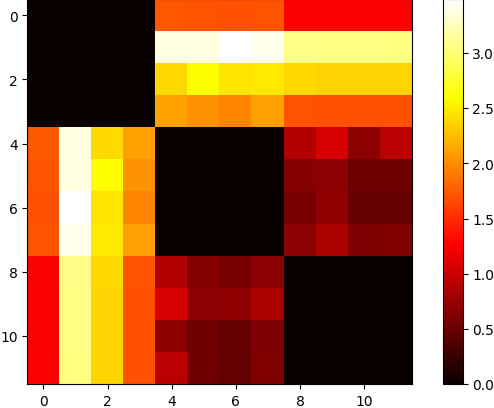
\includegraphics[width=0.6\linewidth]{figures/syntetic_data/distance_matrix/SO3_interpolation}
    \caption[Classification using interpolation to reparameterization of curves in \(\mathrm{SO}(3)\)]{Classification of synthetic \(\mathrm{SO}(3)\) curves across 100 timesteps, with geodesic interpolation to reparameterize, depicted as a distance matrix of twelve curves, denoted \(c_i^j\), where \(i = 1, 2, 3\) and \(j = 1, 2, 3, 4\). The color intensity within the matrix indicates the shape space distance.}
    \label{fig:classification-SO3-interpolation}
\end{figure}

\begin{figure}[!ht]
    \centering
    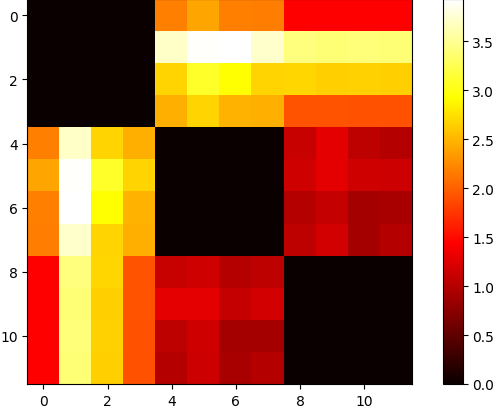
\includegraphics[width=0.6\linewidth]{figures/syntetic_data/distance_matrix/SE3_interpolation}
    \caption[Classification using interpolation to reparameterization of curves in \(\mathrm{SE}(3)\)]{Classification of synthetic \(\mathrm{SE}(3)\) curves across 100 timesteps, with geodesic interpolation to reparameterize, illustrated as a distance matrix of twelve curves, denoted \(c_i^j\), where \(i = 1, 2, 3\) and \(j = 1, 2, 3, 4\). The color intensity within the matrix indicates the shape space distance.}
    \label{fig:classification-SE3-interpolation}
\end{figure}

\FloatBarrier
As seen in the heatmaps, the classification is successful, with almost zero intra-class distances and high inter-class distances. This indicates that the curves are well separated in the shape space, and the classification is accurate. While these results are promising, we refrain from using this method for classifying motion capture data due to uncertainties about its robustness.

% \section{Summary}
\label{subsec:summary-reparam}
Summarize the key points discussed, reflect on the implications of optimal reparametrization, and suggest directions for future research.

